\documentclass[11pt,a4paper]{article}

\usepackage[utf8]{inputenc}
\usepackage[T1]{fontenc}
\usepackage{lmodern}
\usepackage[spanish,es-tabla,es-nodecimaldot,es-noquoting]{babel}
\usepackage{microtype}
\usepackage[margin=2.5cm]{geometry}
\usepackage{amsmath}
\usepackage{graphicx}
\usepackage{booktabs}
\usepackage{threeparttable}
\usepackage{siunitx}
\sisetup{
  output-decimal-marker = {,},
  group-separator = {.},
  group-minimum-digits = 4,
}
\usepackage[font=small,labelfont=bf]{caption}
\usepackage{xcolor}
\usepackage{csquotes}
\usepackage[backend=biber,style=authoryear,maxcitenames=2,uniquelist=false,giveninits=true]{biblatex}
\addbibresource{referencias.bib}
\usepackage[hidelinks]{hyperref}

\graphicspath{{figuras/}}

% Marca visible para todo lo que falta antes de entregar.
\newcommand{\todo}[1]{\textcolor{red}{\textbf{[PENDIENTE: #1]}}}

\title{Priorización de inspecciones de fraude eléctrico a partir del historial de
  facturación: señal de comportamiento frente a huellas de la inspección}
\author{Omar Medina \and Rubén Esguerra\\[4pt]
  \small Seminario de investigación, Programa de Ciencia de Datos, Universidad del Norte}
\date{Noviembre de 2026}

\begin{document}

\maketitle

\begin{abstract}
\noindent\textbf{Introducción.} Las pérdidas no técnicas de energía se combaten con
inspecciones de campo de capacidad limitada, de modo que el problema práctico es decidir a
quién inspeccionar primero. La literatura reporta desempeños muy altos sin controlar que la
etiqueta registra fraude detectado y no fraude cometido.
\textbf{Objetivo.} Desarrollar un modelo de clasificación que ordene a los clientes según su
probabilidad de fraude a partir de su historial de facturación y sus atributos, para
priorizar inspecciones.
\textbf{Métodos.} Se usaron los datos públicos de la empresa tunecina STEG: 135.493 clientes
y 4.476.749 facturas, con 5,58\,\% de fraude detectado. El 20\,\% de los clientes se reservó
como conjunto de prueba evaluado una sola vez, y sobre el resto se aplicó validación cruzada
de cinco pliegues estratificada y agrupada por cliente. El historial de cada cliente se
censuró en su primer reemplazo de contador o cambio de código o de tarifa, por ser huella de
la inspección. Se compararon regresión logística, LightGBM y XGBoost con PR-AUC, ROC-AUC y
precisión en listas de tamaño fijo.
\textbf{Resultados.} Con el historial completo, las variables de su segunda mitad alcanzaron
un PR-AUC de 0,396 frente a 0,182 de la primera; con el historial censurado la diferencia
bajó a 0,032. El modelo seleccionado, LightGBM, obtuvo en el conjunto de prueba un PR-AUC de
0,191 (IC 95\,\% [0,174; 0,211]) y un ROC-AUC de 0,762, frente a 0,132 y 0,745 de una línea
base de exposición. En una lista del 1\,\% de los clientes encontró 118 fraudes, frente a 57
de esa línea base y 15 esperados al azar.
\textbf{Conclusiones.} El historial de facturación permite priorizar inspecciones con una
precisión 7,8 veces superior al azar. Evaluar sin retirar las huellas de la inspección
sobrestima el desempeño que un modelo tendría con clientes aún no inspeccionados.

\medskip\noindent\textbf{Palabras clave:} pérdidas no técnicas; detección de fraude;
priorización de inspecciones; fuga de información; \textit{gradient boosting}.
\end{abstract}

\section{Introducción}\label{sec:introduccion}

Una parte de la energía que entregan las empresas distribuidoras se consume sin pagarse.
Son las pérdidas no técnicas: conexiones directas a la red, medidores manipulados y lecturas
o registros alterados \parencite{glauner2017}. A diferencia de las pérdidas técnicas, que se
disipan en el transporte, estas tienen un origen identificable en el cliente, y su costo
termina recayendo sobre los usuarios que sí pagan.

En Colombia el problema se concentra en la región Caribe, que en junio de 2024 representó
el 28,5\,\% de la demanda nacional de energía eléctrica, según datos de XM
\parencite{elheraldo2024}. En los barrios eléctricamente subnormales que atiende Afinia, la
empresa recauda apenas el 5\,\% de lo que factura, lo que equivale a pérdidas superiores a
300.000 millones de pesos al año \parencite{portafolio2025}. En Air-e, el recaudo acumulado
de 2025 fue del 74,55\,\%, frente a un promedio nacional del 95\,\% \parencite{elheraldo2025}.
Las cifras de recaudo mezclan el fraude con la simple falta de pago, pero dan una idea de la
escala del problema en las distribuidoras de la región.

La respuesta habitual de las empresas es la inspección en campo. Cada visita tiene un costo
y la capacidad de inspección es finita, así que la pregunta operativa es a quién visitar
primero. Por eso el problema se plantea aquí como una tarea de
clasificación orientada a la priorización: ordenar a los clientes según su probabilidad de
fraude a partir de la única información que la empresa tiene de todos ellos, el historial
de facturación y los atributos del contrato.

Ese planteamiento choca con una dificultad que la literatura suele pasar por alto. La
etiqueta de fraude solo existe para los clientes que fueron inspeccionados y en los que se
confirmó el fraude, de modo que mide fraude \emph{detectado}. Un cliente con un historial
largo ha tenido más ocasiones de ser inspeccionado, y una inspección exitosa deja rastros en
el propio historial, como el reemplazo del contador. Un modelo puede aprender esos rastros y
obtener cifras altas en validación sin capacidad real de anticipar el fraude en clientes que
todavía no han sido visitados, que es justamente el uso para el que se construye.

El estudio usa los datos públicos de la Société Tunisienne de l'Électricité et du Gaz
(STEG), liberados en una competencia de la plataforma Zindi \parencite{zindi2019}. Es uno de
los pocos conjuntos abiertos con etiqueta de fraude por cliente y con el historial de
facturación de contadores convencionales, la misma información disponible para las
distribuidoras que no cuentan con medición inteligente. El aporte que se busca tiene dos
partes: un modelo que priorice inspecciones con una mejora medible sobre el azar y sobre una
regla de exposición, y una evaluación que separe la señal de comportamiento del cliente de
la huella que deja la inspección.

\section{Antecedentes y marco teórico}\label{sec:marco}

\subsection{Detección supervisada de pérdidas no técnicas}

La detección de fraude eléctrico con aprendizaje automático tiene unos quince años de
desarrollo. \textcite{nagi2010} sustituyeron la selección de clientes por reglas manuales con
un clasificador de máquinas de vectores de soporte entrenado sobre perfiles de consumo, en
una distribuidora de Malasia. \textcite{comapuig2016} trabajaron con boosting de gradiente
sobre clientes de una empresa española y evaluaron el modelo por campañas de inspección, es
decir, por cuántos fraudes encuentra cada lista que se entrega a los técnicos. En Ecuador,
\textcite{ariasmarin2025} compararon varios clasificadores sobre los datos de una
distribuidora y obtuvieron el mejor resultado con boosting (CatBoost, exactitud de 0,897 y
F1 de 0,894), aunque midieron el desempeño sobre una base de 27.374 registros balanceada
artificialmente entre casos con y sin fraude.

Sobre los mismos datos de STEG que usa este trabajo, \textcite{oprea2022} construyeron
cerca de doscientas variables con funciones analíticas de ventana sobre el historial de
facturas y redujeron el conjunto a quince por puntaje de Fisher. En su escenario de
referencia el mejor AUC fue 0,7331; con la ingeniería de variables propuesta reportan un
AUC de 0,997 para un árbol de decisión. El salto no tiene explicación en el texto, las
variables de ventana se calculan sobre el conjunto completo antes de separar entrenamiento y
prueba, la evaluación descansa en un único corte aleatorio y las quince variables finales no
se nombran. Esas cifras no pueden tomarse como referencia de lo alcanzable. La propia
competencia de Zindi, evaluada con AUC, tuvo un liderato público cercano a 0,86, bajo un
protocolo distinto y sin documentación metodológica publicada por los participantes.

\subsection{La etiqueta depende de la inspección}

En estos conjuntos de datos la etiqueta positiva proviene de una inspección que confirmó el
fraude. \textcite{comapuig2022} hacen de esa procedencia el eje de su trabajo con los datos
de Naturgy: las campañas se dirigen a quien ya parece sospechoso, por lo que el conjunto
etiquetado no representa a la población que se va a puntuar. Documentan un clasificador cuyas
ocho variables más influyentes eran casi todas historial de visitas, es decir, un modelo que
había aprendido el proceso de inspección. \textcite{glauner2016} señalan el mismo sesgo y su
interacción con el desbalance de clases.

De ahí se derivan dos mecanismos que este trabajo mide en sus propios datos. El primero es
la exposición: un cliente con más historial ha tenido más oportunidades de ser
inspeccionado y, por tanto, de ser etiquetado como fraude. El segundo es la huella: si la
inspección confirma el fraude, la empresa reemplaza el contador o modifica el contrato, y esos
cambios quedan en el historial que luego se usa para construir variables.

\subsection{Fuga de información}

Hay fuga cuando el modelo se entrena con información que no estaría disponible en el momento
de predecir \parencite{kaufman2012}. En este problema aparece de dos formas. Una es
procedimental: calcular estadísticos que comparan a un cliente con otros, o escalar y
codificar, usando también los clientes de prueba antes de partir, que es el patrón observado
en \textcite{oprea2022}. La otra es temporal. Como la etiqueta no tiene fecha, cualquier
variable calculada sobre el historial completo puede incluir lo ocurrido después de la
detección, que no existe cuando se puntúa a un cliente todavía no inspeccionado.

\subsection{Métricas para una lista de inspección}

Con una clase minoritaria del 5,58\,\%, un clasificador que nunca predice fraude acierta el
94,42\,\% de las veces, por lo que la exactitud no informa nada. El ROC-AUC mide la
separación global entre clases y no depende de la prevalencia, lo que lo hace adecuado para
comparar subgrupos con tasas de fraude distintas. El PR-AUC, calculado como precisión media,
concentra su peso en la parte alta del ordenamiento, que es donde opera una lista de
inspección, y su valor de referencia al azar es la prevalencia \parencite{saito2015}.

Para una lista con los $k$ clientes de mayor puntuación, con $P$ positivos en la población
y $N$ clientes en total, se usan
\begin{equation}
  \text{precisión@}k = \frac{\text{TP}_k}{k}, \qquad
  \text{recall@}k = \frac{\text{TP}_k}{P}, \qquad
  \text{lift@}k = \frac{\text{precisión@}k}{P/N},
\end{equation}
donde $\text{TP}_k$ es el número de fraudes dentro de la lista. Una lista de tamaño $k < P$
no puede recuperar todos los fraudes, así que el recall@$k$ se compara con su techo
$\min(k, P)/P$ y no con la unidad.

\subsection{Modelos e interpretabilidad}

Los modelos de boosting de gradiente sobre árboles combinan de forma aditiva árboles poco
profundos, cada uno ajustado al error de los anteriores. LightGBM \parencite{ke2017} y XGBoost
\parencite{chen2016} son sus implementaciones más usadas en datos tabulares; ambas toleran
valores faltantes sin imputar y admiten variables categóricas de forma nativa, dos
propiedades relevantes cuando muchos clientes no tienen contador de gas o tienen historiales
cortos. La regresión logística con regularización L2 sirve como referencia lineal.

Para interpretar el modelo se usan los valores SHAP, que reparten la predicción de cada
cliente entre sus variables de forma aditiva \parencite{lundberg2017}; en modelos de árboles
pueden calcularse de manera exacta \parencite{lundberg2020}. Los intervalos de confianza de
las métricas se obtienen por bootstrap \parencite{efron1979} remuestreando clientes, y los de
proporciones del análisis exploratorio con el método de \textcite{wilson1927}.

\subsection{Vacío que aborda este trabajo}

Las técnicas de clasificación avanzaron desde las máquinas de vectores de soporte hasta el
boosting, pero los trabajos revisados rara vez evalúan con la distribución real de clases,
no verifican si la etiqueta depende de la inspección y, en el único antecedente publicado
sobre estos datos, no controlan la fuga. Ninguno separa la parte del desempeño que procede
del comportamiento del cliente de la que procede del rastro de la inspección. Este trabajo
mide esa separación sobre los datos de STEG y evalúa el modelo como se usaría: en listas de
tamaño fijo y frente a referencias simples.

\section{Objetivos, pregunta guía e hipótesis}\label{sec:objetivos}

\subsection{Objetivo general}

Desarrollar un modelo de clasificación que identifique a los clientes de STEG con mayor
probabilidad de fraude detectado, a partir de su historial de facturación entre 2005 y 2019
y de sus atributos, para priorizar las inspecciones de campo.

\subsection{Objetivos específicos}

\begin{enumerate}
  \item Caracterizar los datos de clientes y facturas en cuanto a su calidad, el desbalance
    de clases y la relación entre la longitud del historial y la tasa de fraude.
  \item Construir variables por cliente y comparar modelos de clasificación con una
    validación cruzada agrupada por cliente y un conjunto de prueba sellado, de forma que no
    haya fuga de información.
  \item Evaluar el modelo seleccionado como se usaría en la práctica, midiendo cuántos
    fraudes encuentra una lista de inspección de tamaño fijo frente al azar y frente a una
    línea base de exposición, e interpretar qué variables pesan más en sus predicciones.
\end{enumerate}

\subsection{Pregunta guía}

¿Permite el historial de facturación ordenar a los clientes según su probabilidad de fraude
detectado mejor que el azar y que una referencia basada solo en la exposición a inspección,
una vez se retiran del historial las huellas que deja la propia inspección?

\subsection{Hipótesis}

\begin{description}
  \item[H1.] Una parte del desempeño que se obtiene con el historial completo procede de
    registros posteriores a la detección. Si es así, las variables calculadas sobre la
    segunda mitad del historial rinden claramente más que las de la primera, y esa
    diferencia se reduce al censurar el historial en el primer evento de equipo o de
    contrato.
  \item[H2.] Con el historial censurado, un modelo de boosting sobre variables de
    comportamiento concentra más fraudes en la cabeza de la lista que la línea base de
    exposición, y conserva capacidad de ordenamiento dentro de los clientes que no tuvieron
    ningún evento de equipo o de contrato.
\end{description}

La verificación de H1 quedó registrada como propuesta en la bitácora de decisiones del
proyecto al cerrar el análisis exploratorio, antes de entrenar cualquier modelo.

\section{Metodología}\label{sec:metodologia}

El estudio es cuantitativo, observacional y retrospectivo, con datos secundarios y un diseño
predictivo. La unidad de análisis es el cliente. Todo el proceso está en dos cuadernos
reproducibles del repositorio del proyecto: \texttt{01\_eda.ipynb} para el análisis
exploratorio y \texttt{02\_modelado.ipynb} para la construcción de variables, el
entrenamiento y la evaluación.

\subsection{Datos}

Los datos proceden de STEG y se publicaron en la competencia de Zindi
\parencite{zindi2019}. Se obtuvieron de un espejo público \parencite{kaggle_steg} y se
aceptaron porque los hashes SHA-256 de los cuatro archivos coinciden con los registrados
en el proyecto. La Tabla~\ref{tab:datos} resume su estructura. La tabla de clientes trae el
distrito (4 valores), la categoría del cliente (3), la región (25), la fecha de alta y la
etiqueta. Cada factura registra la fecha, el tipo de tarifa, el número, estado, código y
coeficiente del contador, la nota de lectura, el consumo facturado en cuatro niveles, los
índices anterior y nuevo, el número de meses facturados y el tipo de contador (electricidad
o gas).

% Generado por paper/exportar_artefactos.py desde reports/EDA/00_data_audit.md. No editar a mano.
\begin{table}[htbp]
  \centering
  \small
  \caption{Archivos del conjunto de datos de STEG publicados en el reto de Zindi.}
  \label{tab:datos}
  \begin{threeparttable}
    \begin{tabular}{l S[table-format=7.0] S[table-format=2.0] l}
      \toprule
      {Archivo} & {Filas} & {Columnas} & {Unidad de observación} \\
      \midrule
      \texttt{client\_train} & 135493 & 6 & un cliente con etiqueta \\
      \texttt{client\_test} & 58069 & 5 & un cliente sin etiqueta \\
      \texttt{invoice\_train} & 4476749 & 16 & una factura de un cliente de train \\
      \texttt{invoice\_test} & 1939730 & 16 & una factura de un cliente de test \\
      \bottomrule
    \end{tabular}
    \begin{tablenotes}
      \footnotesize
      \item Solo \texttt{client\_train} trae la etiqueta; \texttt{client\_test} se usa para la validación adversarial.
      \item Fuente: \texttt{reports/EDA/00\_data\_audit.md}.
    \end{tablenotes}
  \end{threeparttable}
\end{table}


Del archivo de clientes de entrenamiento, 7.566 de 135.493 tienen fraude detectado
(5,58\,\%), es decir, 16,9 clientes sin fraude por cada uno con fraude. La etiqueta no tiene
fecha. Los códigos de tarifa, de contador y de nota de lectura carecen de diccionario en la
fuente y el consumo no tiene unidad declarada, por lo que se tratan como categorías sin
interpretar y como magnitud relativa.

\subsection{Calidad y preparación de los datos}

La auditoría de calidad aplicó un catálogo de verificaciones reproducible sobre los cuatro
archivos. No hay valores faltantes en ninguna tabla. Las anomalías se marcaron con
indicadores y no se corrigieron; solo se eliminaron las facturas exactamente duplicadas,
que en el archivo de entrenamiento son 11.
Las anomalías que el conteo no explicaba se investigaron una por una antes de decidir su
tratamiento:

\begin{itemize}
  \item 17.768 de los 18.363 grupos de facturas con la misma clave lógica (cliente, fecha y
    contador) difieren en consumo o en índices, así que no son copias. Se conservaron, porque
    eliminarlas restaría consumo facturado.
  \item 24.043 facturas tienen un número de meses fuera de $[1, 12]$. Entre 13 y 24 meses
    puede tratarse de una regularización real; por encima de mil no admite lectura como
    período. Se marcaron y el consumo mensual solo se calcula para períodos de 1 a 24 meses.
  \item 81 facturas tienen el estado del contador y la nota de lectura desplazados de
    columna en la captura original.
  \item El número de contador se repite en 20.366 valores compartidos por varios clientes,
    así que no identifica un equipo.
  \item 8.748 clientes tienen una primera factura anterior a su fecha de alta, por lo que la
    antigüedad se mide desde la primera factura observada.
\end{itemize}

Los consumos tienen colas extremas, pero la tasa de fraude crece con el consumo máximo del
cliente a lo largo de casi todo su recorrido. Por eso no se truncaron ni se winsorizaron los
valores altos, y el consumo se expresó en escala $\log(1 + x)$.

El historial de facturas va de 1977 a 2019, pero lo anterior a 2005 es el 0,49\,\% de las
facturas. Se fijó una ventana desde el 1 de enero de 2005 para que los clientes fueran
comparables. Esa ventana deja sin ninguna factura a 7.129 clientes cuyo historial es
anterior a 2005; se mantienen en la población con un indicador propio.

\subsection{Análisis exploratorio}

El análisis exploratorio se hizo solo sobre el conjunto de entrenamiento: distribuciones
univariadas por grupos de variables, comportamiento temporal y relación de cada variable con
la etiqueta. Las tasas de fraude por grupo se acompañan de intervalos de Wilson al 95\,\% y
los tamaños de efecto de las variables numéricas se miden con la correlación rango-biserial.
La relación entre la longitud del historial y la tasa de fraude se examinó recalculando cada
efecto dentro de quintiles de número de facturas.

\subsection{Partición y validación}

El conjunto de prueba de Zindi no tiene etiqueta y no sirve para evaluar. Se separó el
20\,\% de los clientes etiquetados, estratificado por la etiqueta y con semilla fija, como
conjunto de prueba sellado (\textit{holdout}): 27.099 clientes que se evaluaron una sola
vez, con el modelo ya elegido. El 80\,\% restante (\textit{dev}, 108.394 clientes con 6.053
positivos) concentró todo el diseño de variables, las comparaciones y la búsqueda de
hiperparámetros.

Sobre \textit{dev} se usó validación cruzada estratificada y agrupada por cliente
(\texttt{StratifiedGroupKFold}) de cinco pliegues, con los mismos pliegues para todos los
modelos, lo que permite comparaciones pareadas. La validación se repitió con otras dos
semillas de partición para medir cuánto depende la cifra del reparto concreto de clientes.

Las variables relativas a pares, la codificación y la transformación de la regresión
logística, y la parada temprana del boosting se ajustan dentro de cada pliegue. La parada
temprana usa un 10\,\% estratificado del pliegue de entrenamiento y nunca el pliegue que se
evalúa. Una validación adversarial, que intenta distinguir con las variables a los clientes
del archivo de entrenamiento de los del archivo de prueba, obtuvo un ROC-AUC de 0,4986: las
variables se calculan y se distribuyen igual en ambos.

\subsection{Censura del historial en el primer evento de equipo o de contrato}

Antes de fijar la representación del historial se verificó si contenía huellas de la
inspección. Se consideraron tres eventos sobre un mismo contador: reemplazo del contador,
cambio de código de contador y cambio de tarifa. Se midió la tasa de fraude con y sin
evento, la posición relativa del evento dentro del historial y cuánto historial queda tras
él. Para contrastar H1 se construyeron las mismas variables con la primera y con la segunda
mitad del historial de cada cliente con al menos 16 facturas, y se compararon sus PR-AUC.

Con esa evidencia (Sección~\ref{sec:res-huellas}) el modelo principal usa el historial
\emph{censurado}: cada cliente conserva solo las facturas anteriores a su primer evento de
equipo o de contrato. La regla no usa la etiqueta, se aplica igual a todos los clientes y
puede aplicarse en el momento de puntuar.

La censura no basta si alguna variable revela \emph{cuándo} se cortó el historial. Varias
magnitudes cambian con el calendario en toda la base, como la codificación de las notas de
lectura o la fracción de consumo en los niveles superiores, de modo que un historial cortado
en un año temprano tiene otro perfil. Las variables con esa deriva se agruparon en dos
conjuntos. El grupo A (notas de lectura y fracción del consumo en niveles superiores) se
retiró, y el grupo B (intervalos largos entre lecturas, estado del contador y códigos de
contador) se conservó, según una regla que retira cada grupo salvo que hacerlo cueste más de
0,005 de ROC-AUC dentro de los clientes sin evento. Esa regla se fijó después de una primera
revisión de fuga, y por eso el modelo sin el grupo B se evalúa también en el conjunto de
prueba como control de sensibilidad.

\subsection{Construcción de variables}

Las variables se calculan por cliente y solo con sus propias facturas, salvo las relativas a
pares, que se ajustan dentro del pliegue. Las de consumo e intervalos se calculan por
separado para electricidad y gas, porque el 45\,\% de los clientes tiene ambos tipos de
contador, con magnitudes de consumo distintas. Se agrupan en familias:

\begin{itemize}
  \item \textbf{Atributos del cliente} (3): región, distrito y categoría, como categorías
    nativas.
  \item \textbf{Nivel de consumo} (8): mediana del log-consumo mensual en las últimas 12
    lecturas, percentil 90, desviación y proporción de lecturas con consumo cero.
  \item \textbf{Dinámica del consumo} (8): pendiente anual del log-consumo, cambio de las
    últimas cuatro lecturas frente a las anteriores y proporción de caídas y subidas fuertes.
  \item \textbf{Regularidad de lectura} (9): intervalos entre lecturas y proporciones de
    facturas con índice que retrocede, duplicado lógico, período anómalo, estado del
    contador distinto de cero e índice inconsistente con el consumo facturado.
  \item \textbf{Tarifa y contador} (10): proporción de facturas de gas y de cada tarifa y
    código de contador frecuente.
  \item \textbf{Relativas a pares} (4): consumo del cliente frente a la mediana de su región
    y de su categoría en el pliegue de entrenamiento.
\end{itemize}

Las proporciones sustituyen a los conteos para que ninguna variable de comportamiento crezca
con la longitud del historial. De las variables candidatas se retiró una por redundancia
($|\rho| > 0{,}95$ de Spearman con otra), además de las del grupo A y de la tasa de cambio de
contador. El modelo final usa 38 variables por cliente y las 4 relativas a pares.

Aparte se construyó una familia de \textbf{exposición} con siete variables: número de
facturas, extensión del historial, antigüedad desde el alta, índice máximo acumulado e
indicadores de primera factura anterior al alta, de historial con menos de 12 facturas y de
ausencia de facturas desde 2005. Estas variables miden oportunidades de
inspección más que propensión a defraudar, así que no entran al modelo principal y se usan
como línea base y como control.

\subsection{Modelos comparados}

\begin{itemize}
  \item \textbf{Prevalencia}: probabilidad constante, equivalente a elegir al azar.
  \item \textbf{Solo exposición}: LightGBM entrenado únicamente con la familia de exposición.
    Representa una regla simple que prioriza a los clientes con más historial.
  \item \textbf{Regresión logística} con regularización L2, codificación \textit{one-hot} y
    transformación por cuantiles ajustadas en el pliegue.
  \item \textbf{LightGBM} con hiperparámetros conservadores (tasa de aprendizaje 0,03, 31
    hojas, 50 clientes mínimos por hoja, submuestreo de filas y columnas) y número de árboles
    fijado por parada temprana \parencite{ke2017}.
  \item \textbf{XGBoost} con una configuración análoga y la misma parada temprana
    \parencite{chen2016}.
  \item \textbf{LightGBM ponderado}, con pesos de clase, como experimento controlado del
    desbalance. No se usó remuestreo.
  \item \textbf{LightGBM con Optuna}: 40 ensayos de búsqueda de hiperparámetros con el
    algoritmo TPE \parencite{akiba2019}, sobre una partición interna de \textit{dev}.
\end{itemize}

Como controles, que no compiten en la selección, se entrenaron el mismo LightGBM sobre el
historial completo y LightGBM con las variables de comportamiento más las de exposición.

La regla de selección se fijó antes de comparar: el mejor modelo es el de mayor PR-AUC fuera
de pliegue, y otro solo se considera peor si el intervalo bootstrap al 95\,\% de la
diferencia excluye el cero y además es peor en al menos 4 de los 5 pliegues. Entre los
indistinguibles se elige el más simple, en el orden regresión logística, LightGBM por
defecto, XGBoost, LightGBM ponderado y LightGBM con búsqueda de hiperparámetros.

\subsection{Métricas y análisis de control}

La métrica principal es el PR-AUC. Se reportan siempre el ROC-AUC, la puntuación de Brier y
la curva de precisión, recall y lift en listas del 0,5, 1, 2, 5 y 10\,\% de los clientes,
porque la capacidad de inspección de la empresa no se conoce. Las diferencias entre modelos
se evalúan con bootstrap pareado por cliente sobre las predicciones fuera de pliegue, y los
intervalos del conjunto de prueba con 1.000 réplicas bootstrap de clientes.

Para separar la señal de comportamiento de la exposición se usan cuatro controles: la
correlación de Spearman entre la puntuación y el número de facturas, el ROC-AUC dentro de
cada quintil de longitud del historial, el desempeño en la población con facturas desde
2005 y el desempeño dentro de los clientes con y sin evento de equipo o de contrato. En el
grupo sin evento no hay corte que delatar, de modo que es la medida más limpia de la señal.

\subsection{Interpretabilidad}

El modelo final se reentrenó con todo \textit{dev}. Sus valores SHAP exactos de árbol se
calcularon sobre una muestra de 20.000 clientes de \textit{dev} \parencite{lundberg2020}.
Esos clientes forman parte del entrenamiento, así que los valores describen qué variables
usa el modelo y no cuánto rinde fuera de muestra.

\subsection{Herramientas y consideraciones éticas}

El análisis se hizo en Python con pandas, scikit-learn \parencite{pedregosa2011}, LightGBM,
XGBoost, Optuna y SHAP, con semillas fijas y versiones registradas en el archivo de
configuración del proyecto. Los datos son públicos y están anonimizados: no contienen
nombres, direcciones ni otra información personal. La puntuación del modelo se interpreta
como la probabilidad de que una inspección confirme fraude y sirve para ordenar visitas;
no constituye una acusación contra el cliente.

\section{Resultados}\label{sec:resultados}

Los resultados se presentan en el orden de los objetivos específicos. Las cifras de
validación cruzada corresponden a \textit{dev} y las del conjunto de prueba sellado, a su
única evaluación.

\subsection{Caracterización de los datos (objetivo específico 1)}\label{sec:res-eda}

El hallazgo central del análisis exploratorio es que la tasa de fraude depende de cuánto
historial tiene el cliente. Entre el decil con menos facturas (1 a 3) y el decil con más (70
a 439) la tasa pasa de 0,642\,\% a 9,756\,\%, un factor de 15,2
(Figura~\ref{fig:historial}). Un historial largo da más ocasiones de inspección, de modo que
parte de lo que un modelo aprendería como señal es exposición acumulada. El número de
contadores del cliente tenía el mayor tamaño de efecto de todas las variables exploratorias
(rango-biserial 0,415) y lo conserva entre 0,22 y 0,40 dentro de cada quintil de longitud
del historial. El índice máximo acumulado, en cambio, cae a $-0{,}015$ en el quintil de
historial más largo: medía exposición y no comportamiento.

\begin{figure}[htbp]
  \centering
  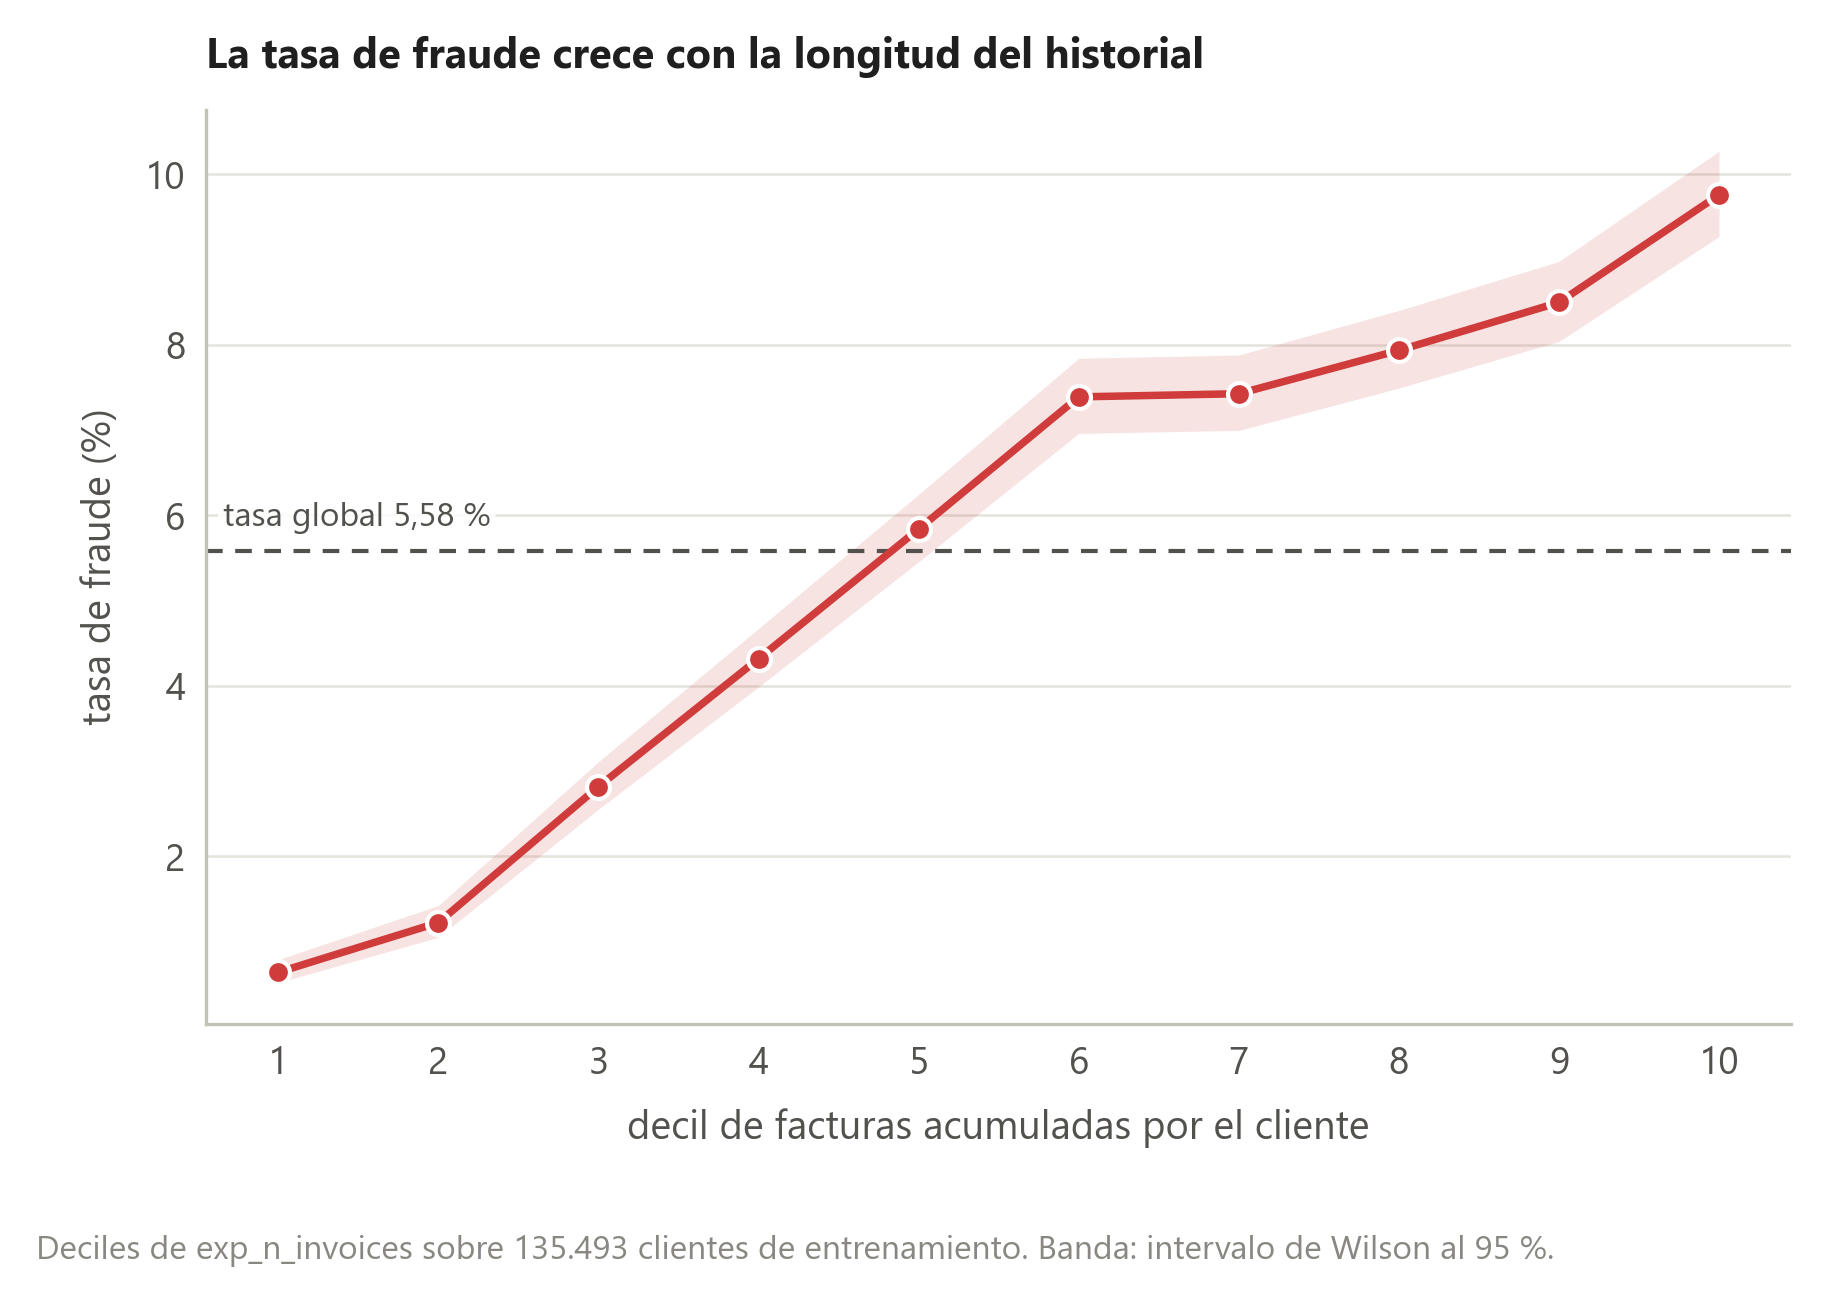
\includegraphics[width=0.72\textwidth]{fig_confusion_historial.png}
  \caption{Tasa de fraude por decil de número de facturas del cliente, con intervalo de
    Wilson al 95\,\%, sobre los 135.493 clientes de entrenamiento.}
  \label{fig:historial}
\end{figure}

El desbalance es marcado pero no hay escasez de casos: 5,58\,\% de positivos, con unos 1.200
positivos en cada pliegue de validación de \textit{dev}. La tasa de fraude también crece con
el consumo máximo del cliente, del 0,649\,\% en el decil más bajo al 11,446\,\% en el más
alto, lo que respalda la decisión de no recortar los consumos extremos.

La Figura~\ref{fig:calidad} resume las anomalías de captura de las facturas. La más
frecuente es el consumo total igual a cero, en el 10,4\,\% de las facturas, seguida de
números de contador iguales a cero y de duplicados por clave lógica. Ninguna afecta a más
del 1\,\% de las filas salvo la primera, y ninguna obligó a descartar clientes. La partición
original de Zindi entre entrenamiento y prueba es aleatoria por cliente: el año de la última
factura se distribuye igual en ambos archivos (V de Cramér corregida 0,003, $p = 0{,}32$).

\begin{figure}[htbp]
  \centering
  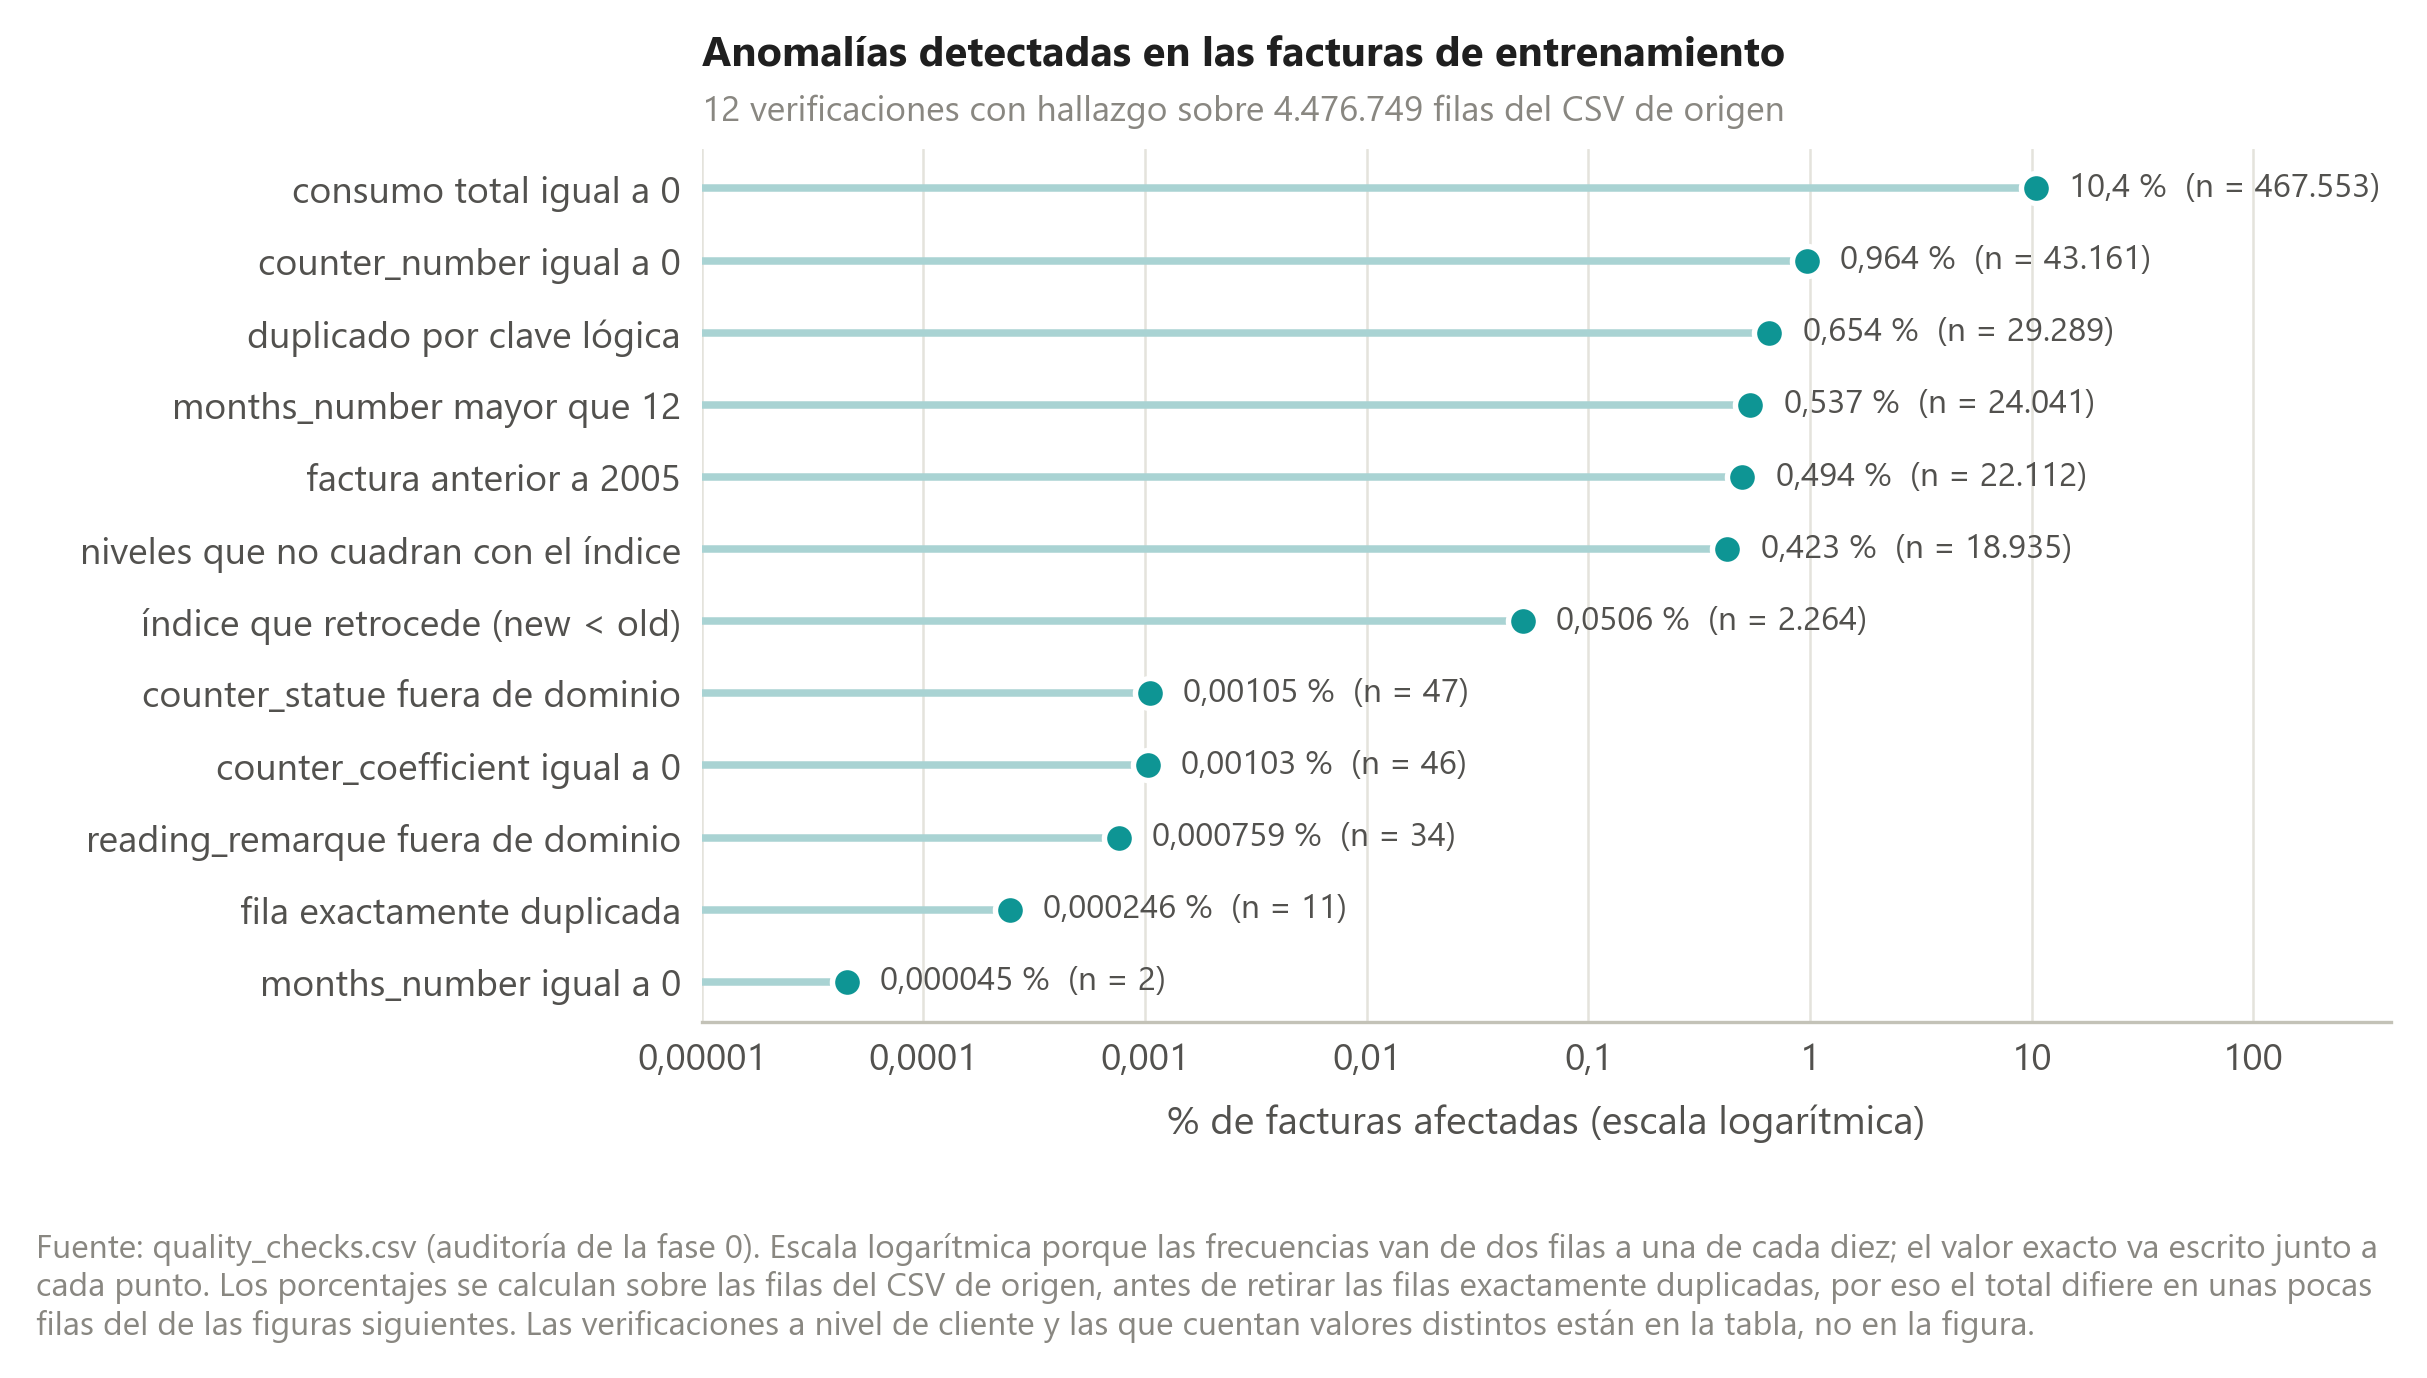
\includegraphics[width=0.9\textwidth]{fig_calidad_anomalias.png}
  \caption{Porcentaje de facturas de entrenamiento afectadas por cada anomalía detectada en
    la auditoría de calidad, en escala logarítmica.}
  \label{fig:calidad}
\end{figure}

\subsection{Variables y comparación de modelos (objetivo específico 2)}

\subsubsection{Huellas de la inspección en el historial}\label{sec:res-huellas}

Los eventos de equipo y de contrato se comportan como consecuencia de la inspección
(Tabla~\ref{tab:eventos}). Los 22.217 clientes de \textit{dev} con alguno de ellos tienen una
tasa de fraude del 18,7\,\%, frente al 2,2\,\% del resto. En los clientes con fraude, el
reemplazo del contador ocurre hacia el final del historial, con una posición relativa
mediana de 0,70 frente a 0,41 en los demás, y después del último reemplazo les quedan 2,7
años de historial frente a 5,7. El código de contador 207 pasa del 7,4\,\% al 10,8\,\% de las
facturas entre la primera y la segunda mitad del historial, y solo en los clientes con
fraude, lo que es compatible con la instalación de un equipo nuevo tras la inspección.

% Generado por paper/exportar_artefactos.py desde reports/tables/modeling_diagnostico_eventos_equipo.csv. No editar a mano.
\begin{table}[htbp]
  \centering
  \small
  \caption{Eventos de equipo y de contrato en el historial de los clientes de \textit{dev}.}
  \label{tab:eventos}
  \begin{threeparttable}
    \begin{tabular}{l S[table-format=5.0] S[table-format=2.1] S[table-format=1.1] S[table-format=1.2] S[table-format=1.2]}
      \toprule
      {Evento} & {Clientes} & {\shortstack{Fraude con\\evento (\%)}} & {\shortstack{Fraude sin\\evento (\%)}} & {\shortstack{Posición\\(fraude)}} & {\shortstack{Posición\\(sin fraude)}} \\
      \midrule
      Reemplazo de contador & 19163 & 18.1 & 2.9 & 0.70 & 0.41 \\
      Cambio de código de contador & 4285 & 26.9 & 4.7 & 0.69 & 0.52 \\
      Cambio de tarifa & 1612 & 17.2 & 5.4 & 0.59 & 0.60 \\
      Cualquiera de los tres & 22217 & 18.7 & 2.2 & 0.69 & 0.47 \\
      \bottomrule
    \end{tabular}
    \begin{tablenotes}
      \footnotesize
      \item Posición: ubicación relativa mediana del evento dentro del historial del cliente (0 = primera factura, 1 = última).
      \item Fuente: \texttt{reports/tables/modeling\_diagnostico\_eventos\_equipo.csv}.
    \end{tablenotes}
  \end{threeparttable}
\end{table}


La verificación por mitades confirma H1 (Tabla~\ref{tab:mitades}). Con el historial
completo, las variables de la segunda mitad alcanzan un PR-AUC de 0,396 y las de la primera
0,182, una diferencia de 0,213 (IC 95\,\% [0,199; 0,227]). Con el historial censurado la
diferencia baja a 0,032 (IC 95\,\% [0,022; 0,041]). La tasa de cambio de contador aporta por
sí sola 0,10 de PR-AUC al modelo con historial completo (0,363 frente a 0,260 sin ella).

% Generado por paper/exportar_artefactos.py desde reports/tables/modeling_verificacion_mitades_historial.csv. No editar a mano.
\begin{table}[htbp]
  \centering
  \small
  \caption{Verificación por mitades del historial: PR-AUC en validación cruzada sobre \textit{dev} con variables calculadas en cada mitad.}
  \label{tab:mitades}
  \begin{threeparttable}
    \begin{tabular}{l l S[table-format=5.0] S[table-format=1.3] c c}
      \toprule
      {Historial} & {Variables de} & {Clientes} & {PR-AUC} & {IC 95\,\%} & {Diferencia con la primera mitad} \\
      \midrule
      Completo & Primera mitad & 74109 & 0.182 & {[0,172; 0,189]} & {---} \\
      Completo & Segunda mitad & 74109 & 0.396 & {[0,381; 0,408]} & {0,213 [0,199; 0,227]} \\
      Completo & Historial entero & 74109 & 0.375 & {[0,362; 0,388]} & {0,194 [0,181; 0,206]} \\
      Censurado & Primera mitad & 64437 & 0.185 & {[0,173; 0,194]} & {---} \\
      Censurado & Segunda mitad & 64437 & 0.217 & {[0,204; 0,225]} & {0,032 [0,022; 0,041]} \\
      Censurado & Historial entero & 64437 & 0.226 & {[0,212; 0,235]} & {0,041 [0,032; 0,049]} \\
      \bottomrule
    \end{tabular}
    \begin{tablenotes}
      \footnotesize
      \item Clientes de \textit{dev} con al menos 16 facturas, para que cada mitad tenga 8 o más; se usan los mismos pliegues restringidos a esa población.
      \item Fuente: \texttt{reports/tables/modeling\_verificacion\_mitades\_historial.csv}.
    \end{tablenotes}
  \end{threeparttable}
\end{table}


\subsubsection{Comparación de modelos}

Con el historial censurado, LightGBM obtiene el mayor PR-AUC en validación cruzada, 0,192
con una desviación de 0,006 entre pliegues, y un ROC-AUC de 0,768 (Tabla~\ref{tab:modelos} y
Figura~\ref{fig:modelos}). XGBoost queda a una diferencia de $-0{,}002$ (IC 95\,\%
[$-0{,}004$; 0,001]) y es indistinguible; por la regla de selección se prefiere LightGBM con
hiperparámetros por defecto. La búsqueda con Optuna y la ponderación de clases dan valores
inferiores en los cinco pliegues, con intervalos que excluyen el cero, así que no se
adoptaron. La regresión logística se queda en 0,131, por debajo de los modelos de boosting y
apenas por encima de la línea base de exposición (0,124). La prevalencia, equivalente al
azar, marca 0,056.

% Generado por paper/exportar_artefactos.py desde reports/tables/model_comparison.csv. No editar a mano.
\begin{table}[htbp]
  \centering
  \small
  \caption{Comparación de modelos en validación cruzada de 5 pliegues sobre \textit{dev} (108.394 clientes, historial censurado).}
  \label{tab:modelos}
  \begin{threeparttable}
    \begin{tabular}{l S[table-format=1.3] S[table-format=1.3] S[table-format=1.3] c S[table-format=1.1]}
      \toprule
      {Modelo} & {PR-AUC} & {Desv.} & {ROC-AUC} & {Diferencia de PR-AUC [IC 95\,\%]} & {Lift@1\,\%} \\
      \midrule
      Prevalencia (azar) & 0.056 & 0.001 & 0.500 & {$-$0,135 [$-$0,145; $-$0,127]} & 1.0 \\
      Solo exposición & 0.124 & 0.005 & 0.732 & {$-$0,068 [$-$0,077; $-$0,060]} & 3.8 \\
      Regresión logística & 0.131 & 0.009 & 0.721 & {$-$0,062 [$-$0,069; $-$0,054]} & 4.3 \\
      XGBoost & 0.190 & 0.007 & 0.767 & {$-$0,002 [$-$0,004; 0,001]} & 6.9 \\
      LightGBM ponderado & 0.185 & 0.009 & 0.763 & {$-$0,007 [$-$0,010; $-$0,004]} & 6.9 \\
      LightGBM con Optuna & 0.187 & 0.008 & 0.766 & {$-$0,004 [$-$0,007; $-$0,001]} & 6.8 \\
      LightGBM (seleccionado) & 0.192 & 0.006 & 0.768 & {---} & 6.7 \\
      \bottomrule
    \end{tabular}
    \begin{tablenotes}
      \footnotesize
      \item PR-AUC y ROC-AUC: media de los 5 pliegues; Desv.: desviación estándar entre pliegues.
      \item Diferencia frente al modelo seleccionado sobre las predicciones fuera de pliegue, con IC por bootstrap pareado por cliente.
      \item Fuente: \texttt{reports/tables/model\_comparison.csv}.
    \end{tablenotes}
  \end{threeparttable}
\end{table}


\begin{figure}[htbp]
  \centering
  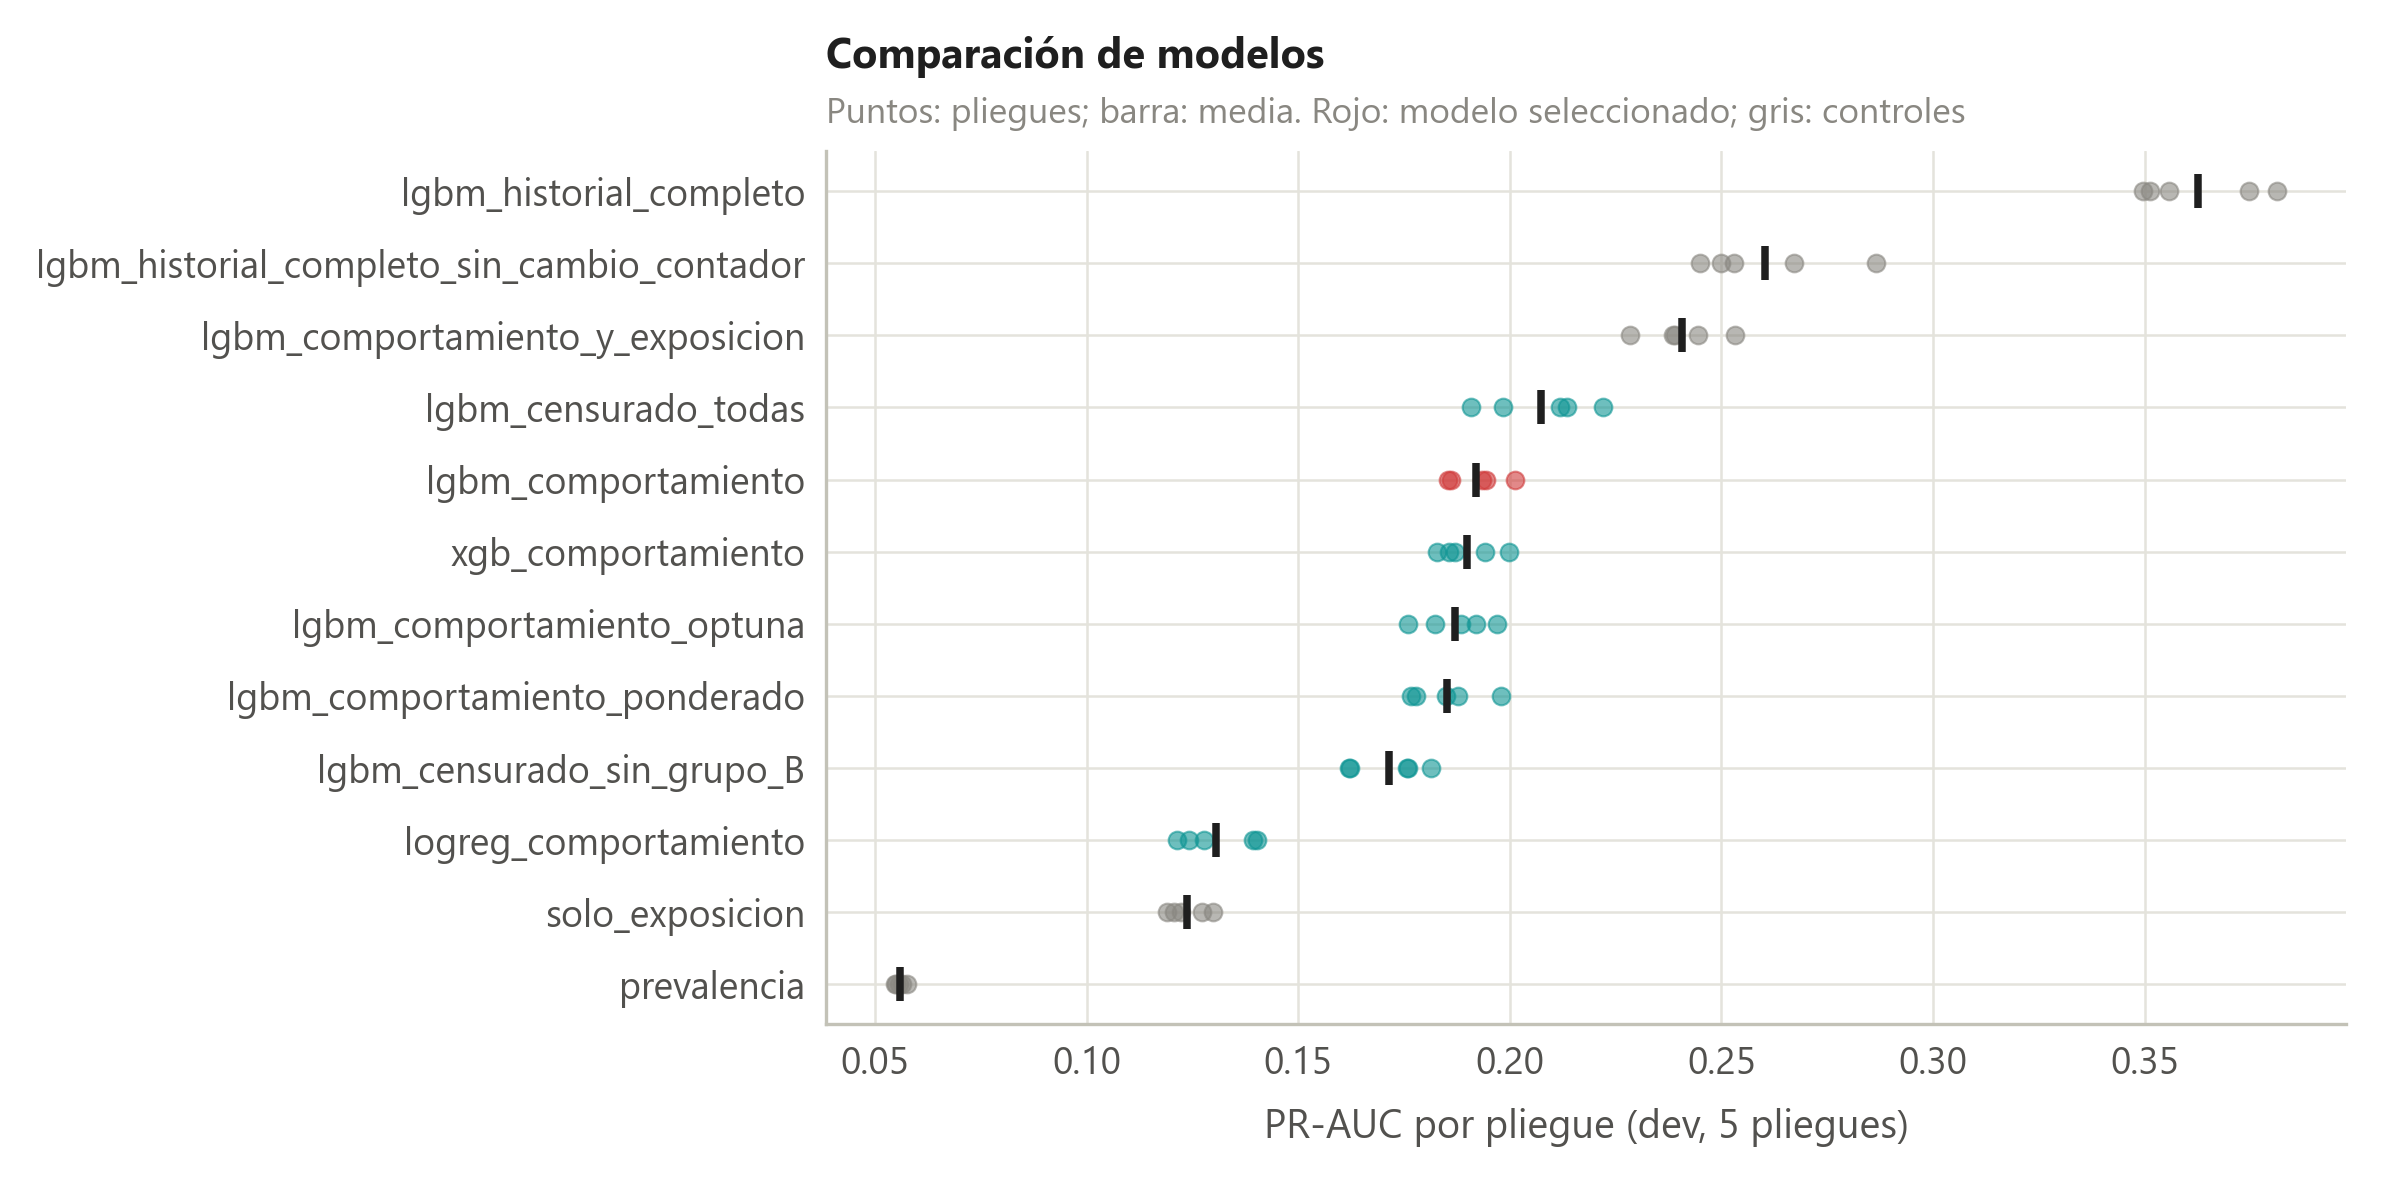
\includegraphics[width=\textwidth]{fig_model_comparacion_pr_auc.png}
  \caption{PR-AUC por pliegue de cada modelo en validación cruzada sobre \textit{dev}. La
    barra marca la media; en rojo el modelo seleccionado y en gris los controles.}
  \label{fig:modelos}
\end{figure}

Los controles muestran cuánto desempeño procede de fuentes que no son el comportamiento del
cliente. El mismo LightGBM con el historial completo llega a 0,363 de PR-AUC y con las
variables de exposición añadidas a 0,241. La puntuación del modelo seleccionado tiene una
correlación de Spearman de 0,42 con el número de facturas, frente a 0,688 de la línea base
de exposición. Dentro de cada quintil de longitud del historial, donde la exposición está
aproximadamente controlada, su ROC-AUC va de 0,707 a 0,775, mientras el de la línea base de
exposición cae de 0,868 en el quintil más corto a 0,632 en el más largo
(Figura~\ref{fig:quintiles}).

\begin{figure}[htbp]
  \centering
  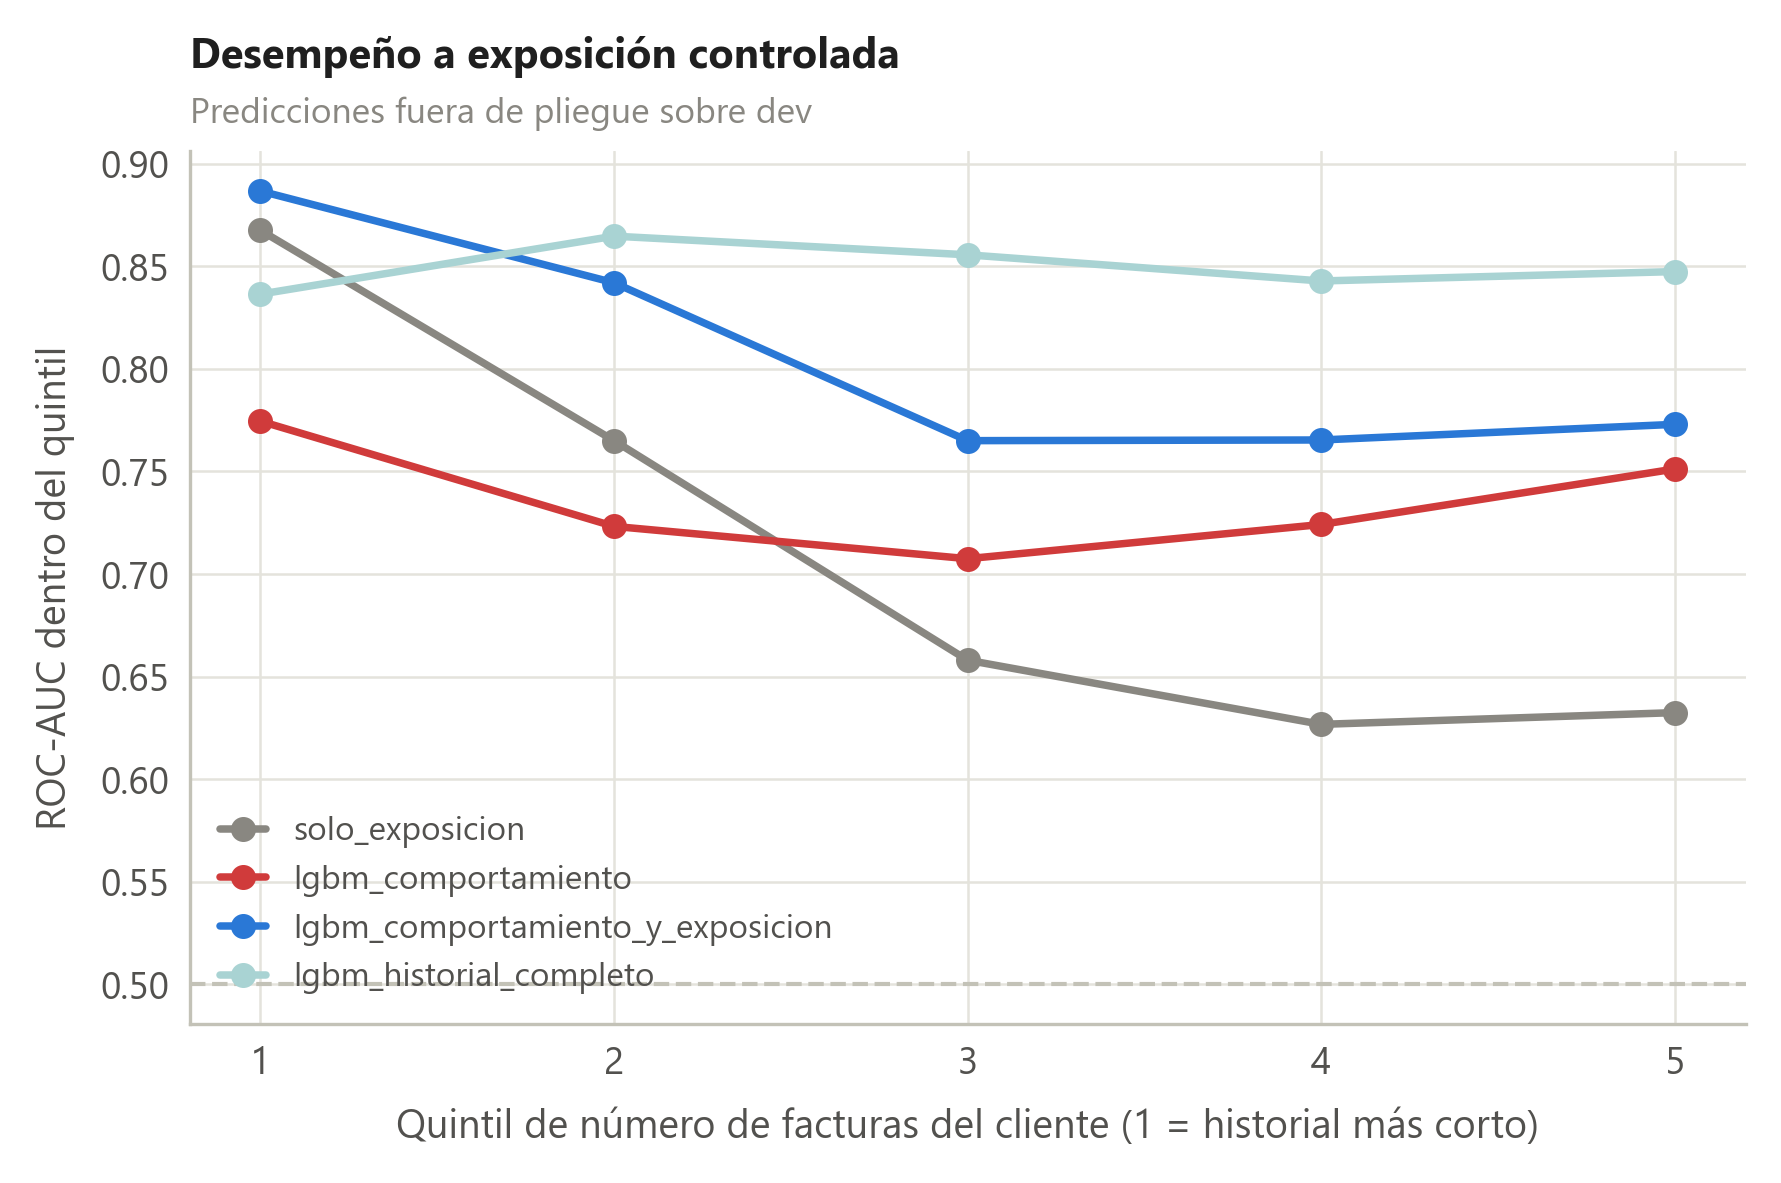
\includegraphics[width=0.75\textwidth]{fig_model_quintiles_historial.png}
  \caption{ROC-AUC dentro de cada quintil de número de facturas, con predicciones fuera de
    pliegue sobre \textit{dev}.}
  \label{fig:quintiles}
\end{figure}

En los 86.177 clientes de \textit{dev} sin ningún evento de equipo o de contrato, con una
prevalencia del 2,2\,\%, el modelo obtiene un ROC-AUC de 0,778 frente a 0,714 de la línea base
de exposición, y un PR-AUC de 0,098. Repetida con otras dos semillas de partición, la
validación cruzada da un PR-AUC medio entre 0,188 y 0,192.

\subsection{Evaluación práctica e interpretación (objetivo específico 3)}

\subsubsection{Desempeño en el conjunto de prueba sellado}

En su única evaluación sobre el conjunto de prueba, el modelo seleccionado obtiene un PR-AUC
de 0,191 (IC 95\,\% [0,174; 0,211]) y un ROC-AUC de 0,762 (IC 95\,\% [0,750; 0,773])
(Tabla~\ref{tab:holdout}). La cifra coincide con la de validación cruzada (0,192), así que el
proceso de selección no produjo un resultado optimista. Supera a la línea base de exposición
en 0,060 de PR-AUC (IC 95\,\% [0,042; 0,077]). El control de sensibilidad sin el grupo B de
variables queda en 0,174 (IC 95\,\% [0,158; 0,192]); aun sin ese grupo, el modelo sigue por
encima de la línea base de exposición, así que la conclusión principal no depende de él.

% Generado por paper/exportar_artefactos.py desde reports/tables/modeling_holdout_metricas.csv. No editar a mano.
\begin{table}[htbp]
  \centering
  \small
  \caption{Desempeño en el holdout sellado (27.099 clientes, 1.513 positivos), evaluado una sola vez.}
  \label{tab:holdout}
  \begin{threeparttable}
    \begin{tabular}{l S[table-format=1.3] c S[table-format=1.3] S[table-format=1.4] S[table-format=2.1] S[table-format=2.1]}
      \toprule
      {Modelo} & {PR-AUC} & {IC 95\,\%} & {ROC-AUC} & {Brier} & {Precisión@1\,\% (\%)} & {Lift@1\,\%} \\
      \midrule
      LightGBM (seleccionado) & 0.191 & {[0,174; 0,211]} & 0.762 & 0.0490 & 43.5 & 7.8 \\
      LightGBM sin grupo B & 0.174 & {[0,158; 0,192]} & 0.742 & 0.0497 & 36.9 & 6.6 \\
      Solo exposición & 0.132 & {[0,122; 0,144]} & 0.745 & 0.0506 & 21.0 & 3.8 \\
      LightGBM con exposición & 0.243 & {[0,223; 0,265]} & 0.818 & 0.0472 & 46.9 & 8.4 \\
      LightGBM historial completo & 0.381 & {[0,359; 0,407]} & 0.879 & 0.0418 & 60.1 & 10.8 \\
      \bottomrule
    \end{tabular}
    \begin{tablenotes}
      \footnotesize
      \item Las dos últimas filas son controles: la exposición mide oportunidades de inspección y el historial completo contiene huellas posteriores a la detección; no son candidatos.
      \item IC del PR-AUC por bootstrap de clientes (1.000 réplicas).
      \item Fuente: \texttt{reports/tables/modeling\_holdout\_metricas.csv}.
    \end{tablenotes}
  \end{threeparttable}
\end{table}


\subsubsection{Fraudes encontrados en una lista de tamaño fijo}

La Tabla~\ref{tab:curva-k} traduce el ordenamiento a campañas de inspección. Si la empresa
visita el 1\,\% de los clientes, 271 en el conjunto de prueba, el modelo encuentra 118 fraudes,
con una precisión del 43,5\,\%. La línea base de exposición encontraría 57 y una selección al
azar, 15. Es una precisión 7,8 veces mayor que la prevalencia y el doble que la de la línea
base. Con listas más largas la precisión baja, como es de esperar, y el lift pasa de 7,3 en el
0,5\,\% a 3,4 en el 10\,\%. Esa lista del 1\,\% recupera el 7,8\,\% de los fraudes, frente a un
techo del 17,9\,\% que impone su tamaño.

% Generado por paper/exportar_artefactos.py desde reports/tables/modeling_holdout_curva_k.csv y modeling_holdout_metricas.csv. No editar a mano.
\begin{table}[htbp]
  \centering
  \small
  \caption{Fraudes encontrados en el holdout según el tamaño de la lista de inspección.}
  \label{tab:curva-k}
  \begin{threeparttable}
    \begin{tabular}{l S[table-format=4.0] S[table-format=3.0] S[table-format=3.0] S[table-format=3.0] S[table-format=2.1] S[table-format=2.1] S[table-format=3.1]}
      \toprule
      {Lista} & {$k$} & {Azar} & {\shortstack{Regla de\\exposición}} & {Modelo} & {\shortstack{Precisión\\(\%)}} & {\shortstack{Recall\\(\%)}} & {\shortstack{Techo de\\recall (\%)}} \\
      \midrule
      0,5\,\% & 135 & 8 & 28 & 55 & 40.7 & 3.6 & 8.9 \\
      1,0\,\% & 271 & 15 & 57 & 118 & 43.5 & 7.8 & 17.9 \\
      2,0\,\% & 542 & 30 & 117 & 192 & 35.4 & 12.7 & 35.8 \\
      5,0\,\% & 1355 & 76 & 234 & 352 & 26.0 & 23.3 & 89.6 \\
      10,0\,\% & 2710 & 151 & 404 & 521 & 19.2 & 34.4 & 100.0 \\
      \bottomrule
    \end{tabular}
    \begin{tablenotes}
      \footnotesize
      \item Azar: prevalencia por $k$. Regla de exposición y modelo: precisión@$k$ por $k$. Precisión, recall y techo corresponden al modelo seleccionado.
      \item Techo de recall: $\min(k, P)/P$, con $P$ = 1.513 positivos del holdout.
      \item Fuente: \texttt{reports/tables/modeling\_holdout\_curva\_k.csv y modeling\_holdout\_metricas.csv}.
    \end{tablenotes}
  \end{threeparttable}
\end{table}


Las probabilidades están calibradas sin necesidad de ajuste (Figura~\ref{fig:holdout},
derecha): en el decil de menor puntuación la probabilidad media predicha es 0,0024 y la tasa
observada 0,0022, y en el decil superior, 0,203 frente a 0,192. La puntuación de Brier es
0,049.

\begin{figure}[htbp]
  \centering
  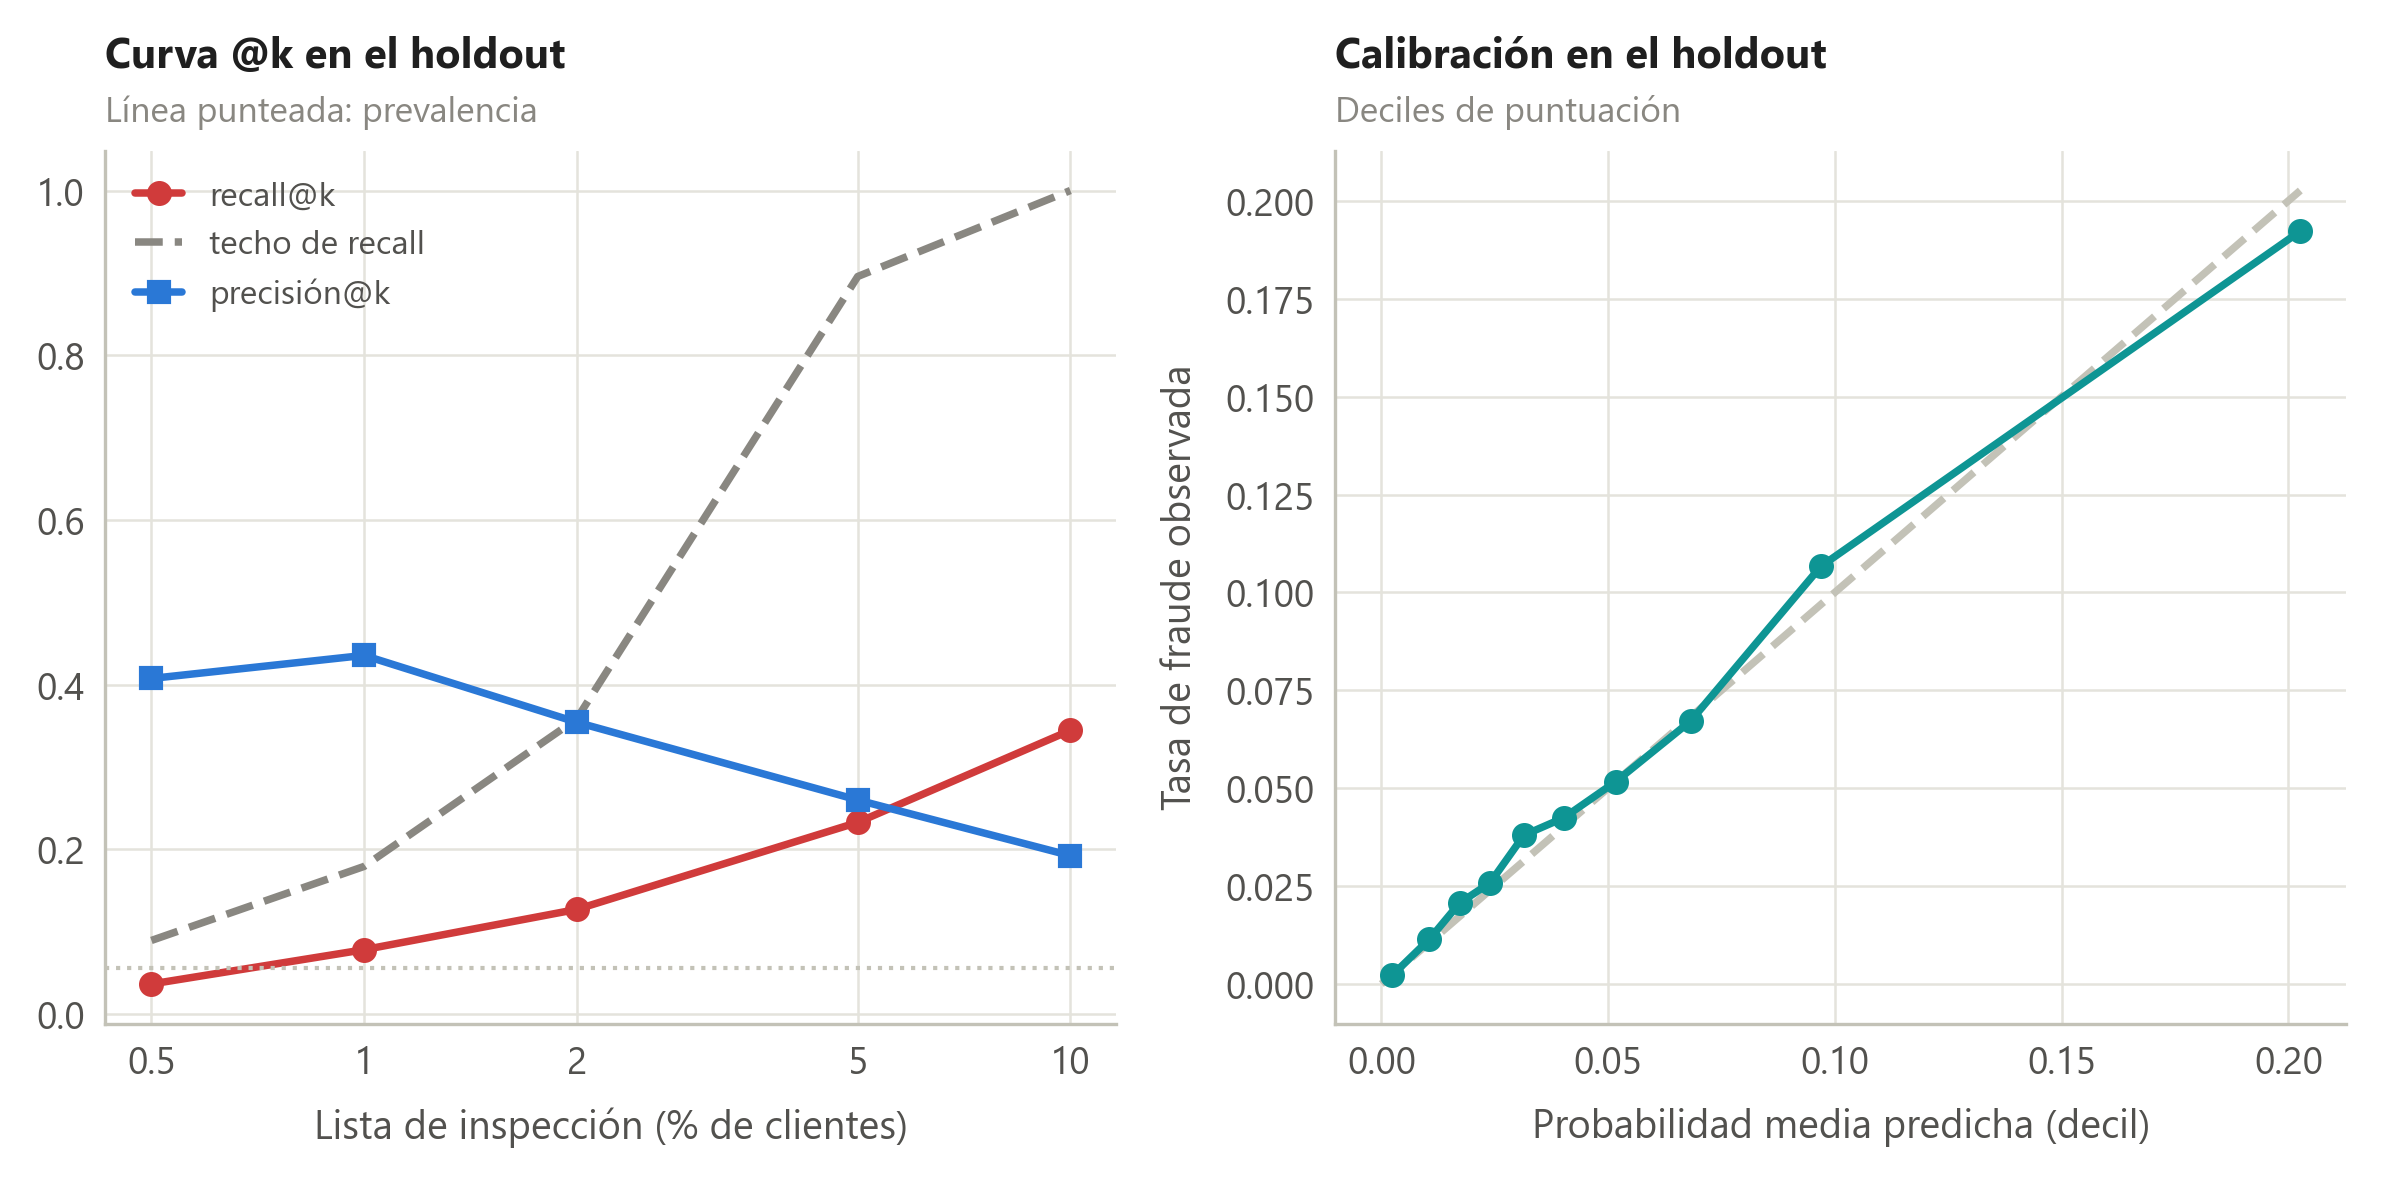
\includegraphics[width=\textwidth]{fig_model_holdout.png}
  \caption{Conjunto de prueba sellado. Izquierda: precisión@$k$, recall@$k$ y techo de recall
    según el tamaño de la lista. Derecha: tasa de fraude observada frente a la probabilidad
    media predicha por decil.}
  \label{fig:holdout}
\end{figure}

\subsubsection{Desempeño por subgrupos}

En los 21.562 clientes del conjunto de prueba sin evento de equipo o de contrato, con una
prevalencia del 2,0\,\%, el modelo obtiene un ROC-AUC de 0,758 y un PR-AUC de 0,086, frente a
0,733 y 0,048 de la línea base de exposición (Tabla~\ref{tab:subgrupos}). La señal se
mantiene donde no hay corte que delatar, como plantea H2. Por quintil de longitud del
historial, el ROC-AUC del modelo en el conjunto de prueba va de 0,676 a 0,798. En el quintil
de historiales más cortos, que solo tiene 54 positivos, la línea base de exposición lo supera
(0,909 frente a 0,798): entre clientes con muy pocas facturas, cuántas tienen sigue
separando a los positivos mejor que su comportamiento. Por distrito, el ROC-AUC va de 0,730
a 0,769.

% Generado por paper/exportar_artefactos.py desde reports/tables/modeling_holdout_por_evento_equipo.csv. No editar a mano.
\begin{table}[htbp]
  \centering
  \small
  \caption{Desempeño en el holdout según el cliente haya tenido o no un evento de equipo o de contrato.}
  \label{tab:subgrupos}
  \begin{threeparttable}
    \begin{tabular}{l S[table-format=5.0] S[table-format=2.1] S[table-format=1.3] S[table-format=1.3] S[table-format=1.3] S[table-format=1.3]}
      \toprule
      {Grupo} & {Clientes} & {Prevalencia (\%)} & {\shortstack{ROC-AUC\\modelo}} & {\shortstack{ROC-AUC\\exposición}} & {\shortstack{PR-AUC\\modelo}} & {\shortstack{PR-AUC\\exposición}} \\
      \midrule
      Sin evento & 21562 & 2.0 & 0.758 & 0.733 & 0.086 & 0.048 \\
      Con evento & 5537 & 19.3 & 0.689 & 0.633 & 0.365 & 0.270 \\
      \bottomrule
    \end{tabular}
    \begin{tablenotes}
      \footnotesize
      \item El grupo sin evento no tiene corte que delatar y da la medida más limpia de la señal de comportamiento.
      \item Fuente: \texttt{reports/tables/modeling\_holdout\_por\_evento\_equipo.csv}.
    \end{tablenotes}
  \end{threeparttable}
\end{table}


\subsubsection{Variables que más pesan}

La familia de tarifa y contador concentra el 31,2\,\% de la contribución SHAP del modelo,
seguida del nivel de consumo (19,6\,\%) y de su dinámica (18,2\,\%)
(Tabla~\ref{tab:shap}). Individualmente, las variables con mayor contribución son la
proporción de facturas con código de contador 207, el percentil 90 del consumo eléctrico, la
región y la pendiente anual del consumo (Figura~\ref{fig:shap}). Los atributos del cliente
aportan el 9,6\,\% y las comparaciones con pares el 7,4\,\%.

% Generado por paper/exportar_artefactos.py desde reports/tables/modeling_importancia_shap.csv. No editar a mano.
\begin{table}[htbp]
  \centering
  \small
  \caption{Participación de cada familia de variables en la media del valor absoluto de SHAP del modelo final.}
  \label{tab:shap}
  \begin{threeparttable}
    \begin{tabular}{l S[table-format=2.0] S[table-format=2.1] l}
      \toprule
      {Familia} & {Variables} & {Participación (\%)} & {Variable con mayor contribución} \\
      \midrule
      Tarifa y contador & 10 & 31.2 & \texttt{inv\_share\_codigo\_contador\_207} \\
      Nivel de consumo & 8 & 19.6 & \texttt{inv\_elec\_log\_cons\_p90} \\
      Dinámica del consumo & 8 & 18.2 & \texttt{inv\_elec\_pendiente\_log\_cons\_anual} \\
      Regularidad de lectura & 9 & 13.9 & \texttt{inv\_share\_estado\_contador\_no\_cero} \\
      Atributos del cliente & 3 & 9.6 & \texttt{cli\_region} \\
      Relativas a pares & 4 & 7.4 & \texttt{rel\_elec\_cons\_vs\_catg} \\
      \bottomrule
    \end{tabular}
    \begin{tablenotes}
      \footnotesize
      \item SHAP calculado sobre 20.000 clientes de \textit{dev}; 42 entradas (38 variables por cliente y 4 relativas a pares).
      \item Fuente: \texttt{reports/tables/modeling\_importancia\_shap.csv}.
    \end{tablenotes}
  \end{threeparttable}
\end{table}


\begin{figure}[htbp]
  \centering
  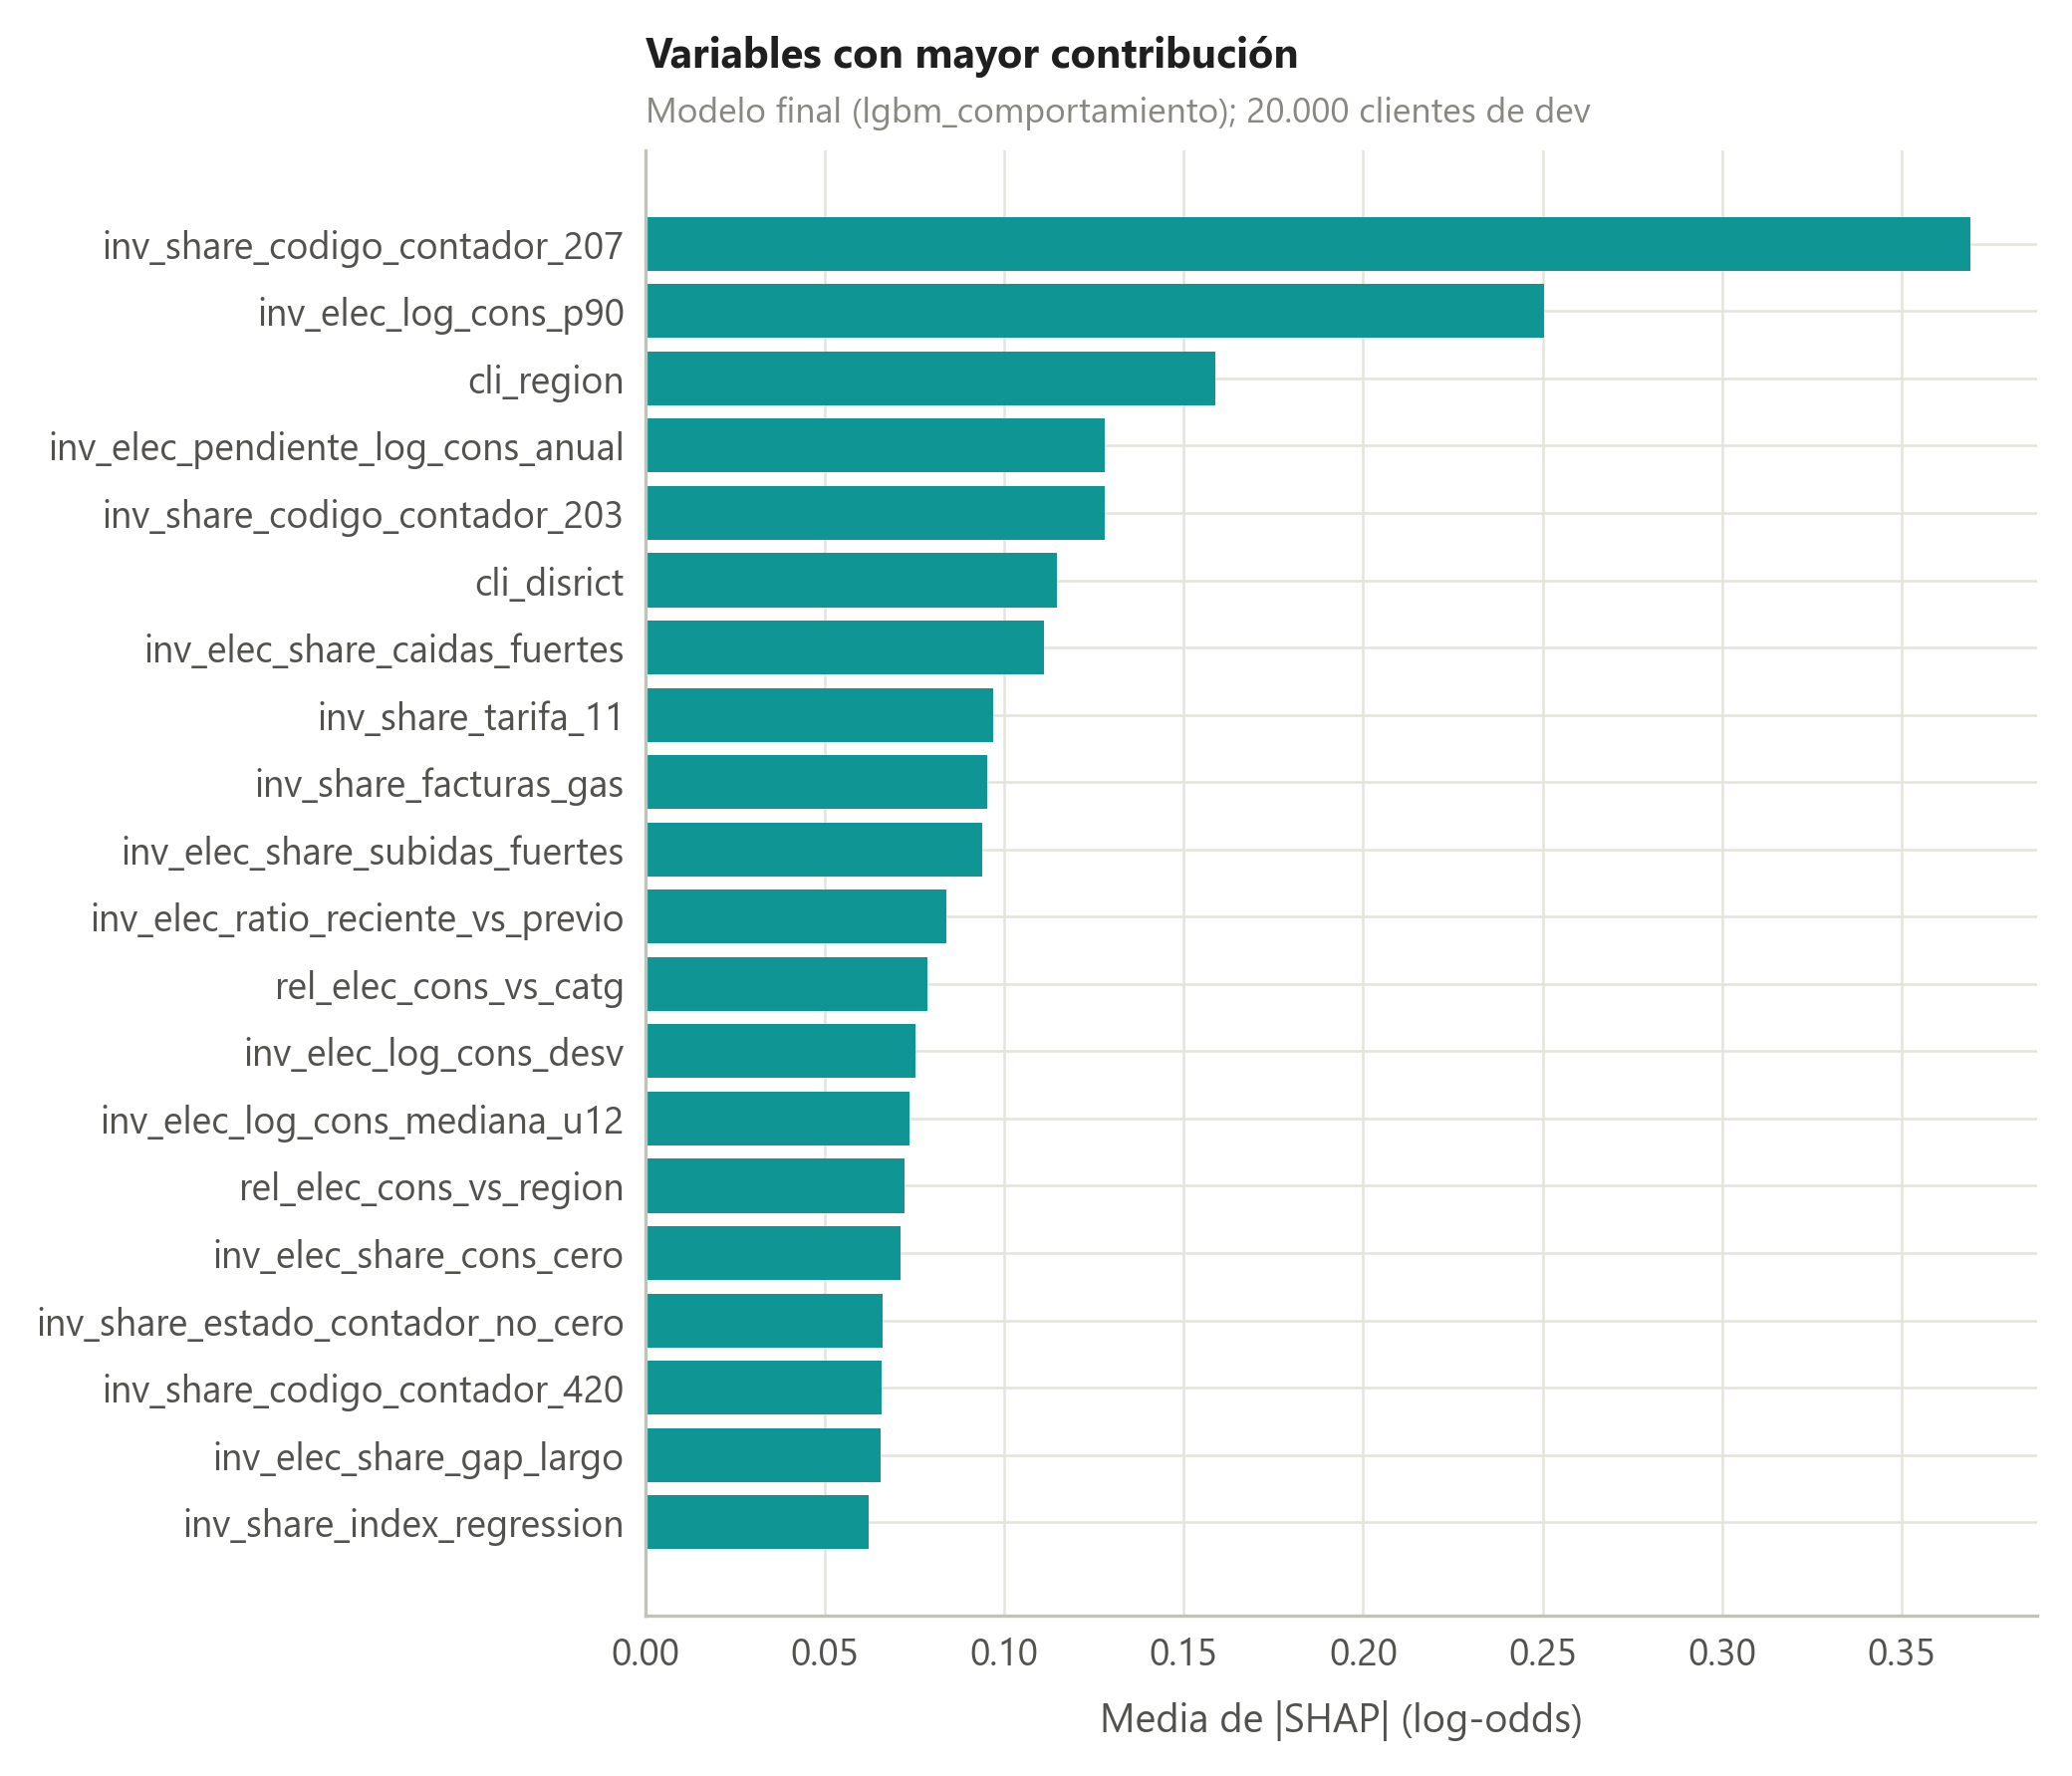
\includegraphics[width=0.8\textwidth]{fig_model_shap_importancia.png}
  \caption{Media del valor absoluto de SHAP de las 20 variables con mayor contribución en el
    modelo final, sobre 20.000 clientes de \textit{dev}.}
  \label{fig:shap}
\end{figure}

\subsection{Respuesta a la pregunta guía}

Las dos hipótesis se sostienen con los datos. H1: la segunda mitad del historial completo
rinde 0,213 más de PR-AUC que la primera, y la censura reduce esa diferencia a 0,032. H2: con
el historial censurado, el modelo encuentra en el 1\,\% superior de la lista el doble de
fraudes que la línea base de exposición y conserva un ROC-AUC de 0,758 entre los clientes sin
eventos. El objetivo general se cumple con un modelo que, sobre clientes que no vio, ordena
con una precisión del 43,5\,\% en la cabeza de la lista frente al 5,58\,\% del azar.

\section{Discusión}\label{sec:discusion}

\subsection{Comparación con la literatura}

El modelo seleccionado rinde por debajo de las cifras publicadas sobre estos datos: un
ROC-AUC de 0,762 en el conjunto de prueba frente al 0,997 de \textcite{oprea2022} y al
liderato cercano a 0,86 de la competencia de Zindi. La diferencia se explica en buena parte
por lo que mide cada cifra. El control entrenado con el historial completo, con el mismo
algoritmo y las mismas precauciones de partición, alcanza en el conjunto de prueba un ROC-AUC
de 0,879 y una precisión del 60,1\,\% en el 1\,\% superior de la lista, una cifra cercana a
la del liderato. La verificación por mitades muestra de dónde sale esa ventaja: la
segunda mitad del historial, la que contiene lo ocurrido después de la detección, rinde más
del doble que la primera. Esa parte del desempeño no existiría al puntuar clientes que
todavía no han sido inspeccionados.

En el caso de \textcite{oprea2022} se suma una segunda fuente probable de optimismo, porque
las variables de ventana se calcularon sobre el conjunto completo antes de partirlo. Con los
datos disponibles no es posible separar cuánto de su 0,997 corresponde a cada mecanismo,
pero la combinación de un único corte aleatorio con variables calculadas sobre todos los
clientes impide tomar esa cifra como referencia.

El hallazgo coincide con el de \textcite{comapuig2022} en datos de otra empresa y otro país:
un clasificador entrenado con etiquetas de inspección termina aprendiendo el proceso de
inspección. Los datos de STEG no traen un historial explícito de visitas; aquí la huella
apareció en cambios administrativos del contador y del contrato, que se registran como
cualquier otra factura. La consecuencia práctica es la misma: sin un control específico,
la validación cruzada premia al modelo que mejor reconoce a los clientes ya inspeccionados.

\subsection{Qué aprendió el modelo}

La variable con mayor contribución es la proporción de facturas con código de contador 207.
Es también la que más dudas plantea, porque ese código gana presencia en la segunda mitad del
historial de los clientes con fraude y se asocia con equipos más recientes. Tras la censura,
las variables del modelo todavía permiten predecir si el cliente tendrá un evento de equipo o
de contrato con un ROC-AUC de 0,871. Parte de la señal, por tanto, puede seguir anticipando
la inspección en lugar del fraude. El resultado en el grupo sin eventos acota ese riesgo: allí
no hay corte que delatar y el modelo mantiene un ROC-AUC de 0,758 en el conjunto de prueba,
por encima de la línea base de exposición.

El nivel y la dinámica del consumo suman el 37,8\,\% de la contribución. El percentil 90 del
consumo eléctrico, la pendiente anual y la proporción de caídas fuertes son variables que
una empresa puede auditar con su propio conocimiento del fraude, algo que no ocurre con un
modelo cuya señal principal fuera la antigüedad del cliente.

\subsection{Limitaciones}

La etiqueta registra fraude detectado y no tiene fecha. Un fraude cometido y nunca
inspeccionado figura como negativo, así que todas las métricas miden la capacidad de
anticipar qué inspección confirmará fraude y no la de detectar fraude cometido. Por la misma
razón no fue posible construir un corte temporal entre historial y etiqueta.

La partición de Zindi es aleatoria por cliente y no cronológica. El desempeño reportado no
mide la capacidad del modelo de generalizar a fraude futuro, que es lo que exigiría su uso en
una campaña real.

La censura es incompleta. Una inspección que confirma fraude sin cambiar el equipo ni el
contrato no deja evento que censurar. Entre las mitades del historial censurado persiste una
diferencia de 0,032 de PR-AUC (IC 95\,\% [0,022; 0,041]), compatible con la mayor relevancia de
lo reciente pero que no descarta un efecto residual de la inspección. La regla que decidió
qué variables con deriva de calendario se retiraban se fijó después de ver una versión
anterior de los resultados; por eso se evaluó el modelo sin el grupo B como control, y su
PR-AUC de 0,174 en el conjunto de prueba sigue por encima de la línea base de exposición.

Los datos son de Túnez. Los códigos de tarifa y de contador no tienen diccionario y el
consumo no tiene unidad, de modo que las variables más importantes no pueden interpretarse
en términos físicos ni trasladarse sin más a otra empresa. Aplicar el método en Colombia
requiere datos de las comercializadoras con la fecha y el resultado de cada inspección.

No se dispuso de costos de inspección ni del valor de la energía recuperada, así que no se
fijó un punto de operación ni se calculó el beneficio neto de cada tamaño de lista. La curva
de la Tabla~\ref{tab:curva-k} es el insumo para ese análisis, que queda pendiente de los
parámetros de costo de la empresa.

\section{Conclusiones}\label{sec:conclusiones}

La introducción planteó una pregunta operativa: con una capacidad de inspección limitada, a
qué clientes visitar primero. El historial de facturación permite responderla mejor que el
azar y mejor que una regla basada en cuánto historial tiene cada cliente. En una campaña que
visita al 1\,\% de los clientes, el modelo propuesto encuentra 118 fraudes donde la selección
al azar encontraría 15 y la regla de exposición 57, y lo hace sobre clientes que no participaron
en ninguna decisión del diseño.

El aporte metodológico es la medición de cuánto desempeño procede de la propia inspección. En
estos datos, el reemplazo del contador y los cambios de código y de tarifa se concentran al
final del historial de los clientes con fraude, y un modelo que los ve alcanza cifras cercanas
a las de la literatura. Al censurar el historial en el primer evento de ese tipo, la ventaja
de la segunda mitad del historial sobre la primera cae de 0,213 a 0,032 de PR-AUC. La cifra
que queda, un PR-AUC de 0,191 y un ROC-AUC de 0,762 en el conjunto de prueba, es la que cabe
esperar al puntuar clientes aún no inspeccionados, y es la que debería guiar una decisión de
uso.

Los tres objetivos específicos se cumplieron. La caracterización de los datos identificó la
longitud del historial como factor de confusión, con una tasa de fraude que se multiplica por
15,2 entre el decil de clientes con menos facturas y el de más. La comparación de modelos, con
pliegues agrupados por cliente, variables relativas ajustadas dentro de cada pliegue y un
conjunto de prueba evaluado una sola vez, seleccionó LightGBM con hiperparámetros por defecto,
indistinguible de XGBoost y mejor que la regresión logística. La evaluación práctica mostró una
precisión del 43,5\,\% en la cabeza de la lista, probabilidades calibradas y una señal que se
mantiene en los clientes sin eventos de equipo o de contrato.

Para trasladar el método a las distribuidoras del Caribe colombiano, la condición más
importante es de registro: conservar la fecha y el resultado de cada
inspección, también de las que no encuentran fraude. Con esa información se puede separar el
historial anterior a la detección del posterior, validar con un corte temporal y fijar el
tamaño de la lista a partir de los costos reales de cada visita.


\printbibliography[title={Referencias}]

\end{document}
